%!TEX TS-program = pdflatex
\documentclass[12pt]{article}  % larger font to compensate for long lines with fullpage
\usepackage{ifpdf,ifxetex}
\ifxetex
% \usepackage{fontspec}
\else % inputenc is incompatible with xetex (which always takes UTF-8 as input)
\usepackage[utf8]{inputenc}
\fi
\usepackage{ifthen}
\usepackage{graphicx}
\usepackage[pdfborder={0 0 0}]{hyperref} % use hyperref without borders
\usepackage{url}
\usepackage{authblk}
\usepackage{longtable}
\usepackage{verbatim}

\newenvironment{XMLexample}
{{\bf Example}\small\verbatim}
{\endverbatim\normalsize}

% Template for GWD/GFD documents.
% Created by Freek Dijkstra, original concept by Bruce Lowekamp.
% This template is placed in the public domain.

% Define some basics for your document:

\title{Usage Record – Format Recommendation}  % Full title of the document
\newcommand{\shortdoctitle}{UR-2.0}  % Title used in page header
\date{\today} %and \author{} %are currently ignored
\newcommand{\authorsshort}{A. Cristofori (editor), IGI Bologna\\
J. K. Nilsen (editor), Univ. of Oslo\\ 
J. Gordon, STFC RAL London\\ 
M. Jones, Univ. of Manchester\\
J. A. Kennedy, RZG Munich\\
R. Müller-Pfefferkorn, TU Dresden
}  % name(s) and institution(s) of corresponing author(s) as shown on the title page.
\newcommand{\publicationdate}{January 2013}  % Date of first publication of the document
% \newcommand{\revisiondate}{December 2010}  % Optional: date of last revision of the document
\newcommand{\copyrightyears}{2006-2013}  % Years used in copyright notice
\newcommand{\docseries}{GFD-R-P.204}  % GWD-R, GWD-I or GWD-C (for working drafts), GFD-I, GFD-R, or GFD-C
\newcommand{\groupname}{UR-WG}  % Optional: name of the authoring working or research group
\newcommand{\groupurl}{\href{mailto:ur-wg@ogf.org}{ur-wg@ogf.org}}  % Optional: URL or email address of the authoring working or research group
\newcommand{\documenturl}{}  % Optional: URL of this document

% Read pictures from img/ and current directory
\graphicspath{{img/}{./}}

%%% GWD/GFD header follows %%%
% Feel free to make changes, as long as your document follows the guidelines of GFP.152

\usepackage[numbers]{natbib} % Use [1] for references, 
\bibliographystyle{unsrtnat} % References show full author name(s) and document URL

\usepackage[sf,compact]{titlesec} % Use sans-serif for section headers

\usepackage[titles]{tocloft} % Format table of contents
% (tocloft is used, since titletoc is incompatible with xetex.)
\renewcommand{\cftsecfont}{\sffamily}
\renewcommand{\cftsubsecfont}{\sffamily}
\renewcommand{\cftsubsubsecfont}{\sffamily}
\renewcommand{\cftsecpagefont}{\sffamily}
\renewcommand{\cftsubsecpagefont}{\sffamily}
\renewcommand{\cftsubsubsecpagefont}{\sffamily}
\renewcommand{\cftsecleader}{\cftdotfill{\cftsubsecdotsep}} % dots for sections the same as for subsections

%\newcommand{\beginXML}{\tiny \begin{verbatim}}
%\newcommand{\endXML}{\end{verbatim} \normalsize}

\setlength{\cftbeforesecskip}{0.5ex}


\usepackage{parskip} % Blank lines between paragraphs, no indentation.

% % Tune placement of figures. (defaults are so strict that images and text are often separated.)
% \renewcommand{\textfraction}{0.05}  % min fraction of page for text. default: 0.2
% \renewcommand{\topfraction}{0.95}   % max fraction of page for floats at top. default: 0.7
% \renewcommand{\bottomfraction}{0.95}% max fraction of page for floats at bottom. default: 0.3
% % \renewcommand{\floatpagefraction}{0.35} % min fraction of floatpage that should have floats. default: 0.5
% % \setcounter{totalnumber}{5}         % max number of floats on a page
% 
% % Tune placement of text. (defaults are not strict enough.)
% \widowpenalty=500% penalty for single line on top of succeeding page. default 150
% \clubpenalty=500% penalty for single line on bottom of preceeding page. default 150
% \tolerance=1000% abort if the penalty exceeds 1000. default infinite.

% font style for text body
% \renewcommand{\familydefault}{\sfdefault}

% font style for headers and footers
\newcommand{\headerstyle}{\sffamily} % sans-serif

% Set page margins
\usepackage{fancyhdr}
\addtolength{\headheight}{15pt}
\renewcommand{\headrulewidth}{0pt}
% \setlength{\headrulewidth}{0pt}
\setlength{\headsep}{20pt}
\usepackage[headings]{fullpage}  % small margins

% Macro to check if (optional) values above are defined or not.
\newcommand{\ifnonempty}[2]{\ifthenelse{\isundefined{#1}}{}{\ifthenelse{\equal{#1}{}}{}{#2}}}

% Define page header and footers
\pagestyle{fancyplain}
\fancyhf{}
\lhead{\fancyplain{}{\headerstyle\docseries}}
% use \revisiondate if defined, otherwise \publicationdate for right header:
\rhead{\fancyplain{}{\headerstyle\ifthenelse{\isundefined{\revisiondate }}{\publicationdate}{\ifthenelse{\equal{\revisiondate}{}}{\publicationdate}{\revisiondate}}}}
\lfoot{\headerstyle\ifnonempty{\groupurl}{\groupurl}}
\rfoot{\headerstyle\thepage}
\thispagestyle{plain}

\begin{document}

% Title page header
{\noindent
\begin{minipage}[t]{3.0in}
\headerstyle
\docseries \\
\ifnonempty{\groupname}{\groupname \\}
\ifnonempty{\groupurl}{\groupurl \\}
\ifnonempty{\documenturl}{\documenturl \\}
\end{minipage}
\hfill
\raggedleft
\begin{minipage}[t]{3.0in}
\raggedleft
\headerstyle
\authorsshort \\
\publicationdate \\
\ifnonempty{\revisiondate}{Revised \revisiondate \\}
\end{minipage}
}

\begin{center}
\makeatletter
\Large\bf\textsf \@title
\makeatother
\end{center}


%%% End of header, insert content below this line %%%

\subsection*{Status of This Document}

% Pick one of the following:
%Group Working Draft (GWD)
GFD-R-P.204
%Grid Final Draft (GFD)
%Grid Recommendation
%Obsolete. This document is replaced by/obsoleted by GFD-I.xxx~\cite{gfd0000}.
%Historical

\subsection*{Obsoletes}
%% include or remove this section if applicable

This document obsoletes GFD-R-P.098\cite{mach2007usagerecord}.

%\subsection*{Document Change History}
%% include or remove this section if applicable

%This template has been updated to confirm to GFD-C.152~\cite{gfd152}.

\subsection*{Copyright Notice}

Copyright \copyright \ Open Grid Forum (\copyrightyears).  Some Rights Reserved.  
Distribution is unlimited.

%\subsection*{Trademark}
%% include or remove this section if applicable

%XXXX is a registered trademark and service mark of the Open Grid Forum. 

\phantomsection\addcontentsline{toc}{section}{Abstract}

This document, part of a document series, produced by the OCCI working
group within the Open Grid Forum (OGF), provides a high-level
definition of a Protocol and API. The document is based upon
previously gathered requirements and focuses on the scope of important
capabilities required to support modern service offerings.



\newpage
\phantomsection\addcontentsline{toc}{section}{Contents}
\tableofcontents

\newpage

%!TEX root = nml-base.tex

\section{Introduction}%
\label{sec:introduction}

This document describes the base schema of the Network Markup Language (NML).
Section~\ref{sub:classes} defines the NML classes and their attributes and parameters.
Section~\ref{sub:relations} describes the relations defined between NML classes.

An NML network description can be expressed in XML\cite{xml}, and RDF/XML\cite{rdfxml} syntax.
Section~\ref{s:xmlschema} describes the XSD schema for the XML syntax.
Section~\ref{s:owlschema} describes the OWL 2 schema for the RDF/XML syntax.

These basic classes defined in this document may be extended, or sub-classed, 
to represent technology specific classes.

Section~\ref{s:examples} provides example use cases. This section is informative. 
Only sections~\ref{s:schema}, \ref{s:identifiers}, \ref{s:syntax}, and appendices \ref{s:xmlschema} and \ref{s:owlschema} are normative and considered 
part of the recommendation.

Appendix~\ref{s:g800terms} is informative and explains the relation between terms defined in this document and those defined in the ITU-T G.800 recommendation~\cite{g800}.

\subsection{Context}
\label{sec:context}

The Network Markup Language (NML) has been defined in the context of research and 
education networks to describe so-called hybrid network topologies. The NML is defined
as an abstract and generic model, so it can be applied for other network topologies as well.
See \cite{gfd.165} for an detailed overview including prior work.

\subsection{Scope}
\label{sec:scope}

The Network Markup Language is designed to create a functional description of 
multi-layer networks and multi-domain networks. An example of a multi-layered 
network can be a virtualised network, but also using different technologies. 
The multi-domain network descriptions can include aggregated or abstracted network topologies.
NML can not only describe a primarily static network topology, but also its potential capabilities (services) 
and its configuration.

NML is aimed at logical connection-oriented network topologies, more precisely topologies
where switching is performed on a label associated with a flow, such as a VLAN, wavelength or time slot. 
NML can also be used to describe physical networks or packet-oriented networks, 
although the current base schema does not contain classes or properties 
to explicitly deal with signal degradation, or complex routing tables.

NML only attempts to describe the data plane of a computer network, not the control 
plane. It does contain extension mechanism to easily tie it with network provisioning 
standards and with network monitoring standards.

Finally, this document omits a definition for the terms \emph{Network} or \emph{capacity}. 
This has been a conscious choice. The term \emph{Network} has become 
so widely used for so many diverse meanings that it is impossible to create a 
definition that everyone can agree on, while still expressing something useful.
See \emph{Topology} for the concept of a network domain and a \emph{Link} with multiple 
sources and sinks for the concept of a local area network.
The term \emph{capacity} is used by different technologies in such a different 
way (e.g.\ including or excluding the header and footer overhead) that it is better 
to let technology-specific extensions make an explicit definition.

\subsection{Notational Conventions}%
\label{sec:rfc2119}

The keywords “\MUST{}”, “\MUSTNOT{}”, “\REQUIRED{}”, “\SHALL{}”, “\SHALLNOT{}”, 
“\SHOULD{}”, “\SHOULDNOT{}”, “\RECOMMENDED{}”, “\MAY{}”,  and “\OPTIONAL{}” are 
to be interpreted as described in \cite{rfc2119}.
% except that the words do not appear in uppercase. 

This schema defines classes, attributes, relations, parameters and logic.
Objects are instances of classes, and the type of an object is a class.

Names of classes are capitalised and written in italics (e.g.\ the \emph{Node} class).
Names of relations are written in camel case and in italics (e.g.\ the \emph{hasNode} relation).
Names of identifiers and string literals are written in monspaces font (e.g. \texttt{Port\_X:in}).

Diagrams in this document follow the diagrammatic conventions of UML class diagrams.
\begin{itemize}
\item A subclass-superclass relationship is represented by a line with hollow triangle shape pointing to the superclass.
\item A whole-part relationship is represented by a line with a hollow diamond shape pointing to the whole (group).
\item A entity-relationship is represented by a line, optionally with numbers at each end indicating the cardinality of the relation. A named entity-relationship has a verb next to the line, and a filled triangle pointing to the object of the verb. (e.g. the entitity-relationship
\nmlrelation{BidirectionalPort}{*}{hasPort}{2}{Port} is named \emph{hasPort}, and each \emph{BidirectionalPort} is related to exactly 2 \emph{Port}s, and each \emph{Port} may be associated with zero, one or more \emph{BidirectionalPort}s.)
\end{itemize}


\newpage
% !TeX root = draft-ur-v2.tex
% encoding=utf-8

\section{Conventions Used in this Document}
\label{s:conventions}

\subsection{Notational Conventions}
\label{s:rfc2119}

The key words ``MUST'' ``MUST NOT'', ``REQUIRED'', ``SHALL'', ``SHALL NOT'', ``SHOULD'', ``SHOULD NOT'', ``RECOMMENDED'', ``MAY'',  and ``OPTIONAL'' are to be interpreted as described in RFC 2119~\cite{rfc2119}, except that the words do not appear in uppercase. 



%%%%%%%%%%%%%%%%%%



\subsection{Meta Properties}

Meta properties are associated with individual base properties to provide additional information and semantic meaning of the value for a base property.  The meta properties outlined below are commonly encountered and should be supported for the indicated base properties.



%%%%%%%%%%%%%%%%%%



\subsubsection{Description}

The description provides a mechanism for additional, optional information to be attached to a Usage Record base property.  The value of this meta-property MAY provide clues to the semantic context to use while interpreting or examining the value of the owning base property.



%%%%%%%%%%%%%%%%%%



\subsubsection{Metric}

This meta-property identifies the type of measurement used for quantifying the associated resource consumption if there are multiple methods to measure resource usage. As an example, disk usage may be measured as total, average, minimum or maximum usage. However, even if pertinent to the assessed charge, this meta-property does not attempt to differentiate between requested and utilized quantities of resource usage.



%%%%%%%%%%%%%%%%%%



\subsubsection{Time Stamps}

Time stamps should follow the ISO 8601\cite{wolf1998date} standard as well. This includes enumerating the time zone, as specified in the standard.



%%%%%%%%%%%%%%%%%%



\subsection{Conventions}

Unless otherwise stated, all fields are optional. A required field is only required if the corresponding block is present.



%%%%%%%%%%%%%%%%%%



\subsection{Supported Data Types}

\begin{enumerate}
\item String: Data of this type has no required restrictions on the length or available characters.
\item Integer
\item Positive integer: Data of this type must have a value of zero or greater.
\item Non-zero integer: Data of this type must have a value of one or greater.
\item Float: Data of this type must be a decimal number.
\item Timestamp: Data of this type must comply with the UTC time zone format specified in ISO 8601.
\item DomainName: Data of this type must comply with RFC 1034\cite{mockapetrisrfc} format for fully qualified domain names.  The constraints are a maximum 255 characters long, containing only alphabetic and numeric characters, the “-“,  and the “.” characters.
\end{enumerate}


%%%%%%%%%%%%%%%%%%
\newpage
% !TeX root = draft-ur-v2.tex

\section{RecordIdentityBlock}

This block contains the properties related to the identity of the usage record itself.

\begin{XMLexample}
<ur:RecordIdentityBlock>
<!— Identity properties go in here -->
</ur:RecordIdentityBlock>
\end{XMLexample}



%%%%%%%%%%%%%%%



\subsection{RecordId}

A record identity uniquely defines a record in the set of all usage records of the accounting context.
\begin{itemize}
\item \emph{RecordId} MUST be present in the \emph{RecordIdentityBlock}.
\item \emph{RecordId} MUST be a string.
\end{itemize}

\begin{XMLexample}
<ur:RecordId>"host.example.org/ur/87912469269276"</ur:RecordId>
\end{XMLexample}



%%%%%%%%%%%%%%%



\subsection{CreateTime}

The time when this particular Usage Record was created.
\begin{itemize}
\item \emph{CreateTime} MUST be present in the \emph{RecordIdentityBlock}.
\item \emph{CreateTime} MUST be an ISO 8601:2004 timestamp.
\end{itemize}

\begin{XMLexample}
<ur:CreateTime>2013-05-09T09:06:52Z</ur:CreateTime>
\end{XMLexample}



%%%%%%%%%%%%%%%



\subsection{Site}

The site at which the resource is located. This property should contain a descriptive name of the group of resources which are accounted for in the record. The \emph{Site} value should be constructed in such a way that it is unique within the context where it is used.
\begin{itemize}
\item \emph{Site} MUST be a string.
\end{itemize}

\begin{XMLexample}
<ur:Site>"ACME-University"</ur:Site>
\end{XMLexample}



%%%%%%%%%%%%%%%



\subsection{Infrastructure}

The infrastructure where the resource was used (e.g., EGI or OSG).
\begin{itemize}
\item \emph{Infrastructure} MUST be a string.
\item The attribute \emph{description} SHOULD be used to give additional information on the used infrastructure.
\end{itemize}

\begin{XMLexample}
<ur:Infrastructure ur:description="U.S Open Science Grid">"OSG"</ur:Infrastructure>
\end{XMLexample}

\newpage
% !TeX root = draft-ur-v2.tex

\section{SubjectIdentityBlock}

This block contains the properties related to the identity of the subject accounted for. 

There are many ways to identify a subject or a group and it depends on the infrastructure used. Thus, all fields in this block are optional. 
A community that wants to exchange usage information has to decide 
on a particular identification.
This should be reflected in a community specific profile associated with this block that defines at least one field that must be present.

\begin{XMLexample}
<ur:SubjectIdentityBlock>
<!— Identity properties go in here -->
</ur:SubjectIdentityBlock> 
\end{XMLexample}



%%%%%%%%%%%%%%%



\subsection{LocalUserId}

The local identity of the user accountable for the resource consumption (e.g., the Unix user).
\begin{itemize}
\item \emph{LocalUserId} MUST be a string.
\end{itemize}

\begin{XMLexample}
<ur:LocalUserId>"johndoe"</ur:LocalUserId> 
\end{XMLexample}



%%%%%%%%%%%%%%%



\subsection{LocalGroupId}

The local group accountable for the resource consumption (e.g., Unix group).
\begin{itemize}
\item \emph{LocalGroupId} MUST be a string.
\end{itemize}

\begin{XMLexample}
<ur:LocalGroupId>"projectA"</ur:LocalGroupId> 
\end{XMLexample}



%%%%%%%%%%%%%%%



\subsection{GlobalUserId}

The global identity of the user accountable for the resource consumption. The property should identify the user globally, such that clashes do not happen accidentally, e.g. it could be an X500 identity.
\begin{itemize}
\item \emph{GlobalUserId} MUST be a string.
\end{itemize}

\begin{XMLexample}
<ur:GlobalUserId>"/O=Grid/OU=example.org/CN=John Doe"</ur:GlobalUserId>
\end{XMLexample}



%%%%%%%%%%%%%%%



\subsection{GlobalGroupId}

The global group accountable for the resource consumption. The property should identify the group globally, such that clashes do not happen accidentally, e.g. using a Fully Qualified Domain Name (FQDN) to construct it. In a Grid context, this would typically be the name of the Virtual Organization (VO).
\begin{itemize}
\item \emph{GlobalGroupId} MUST be a string.
\end{itemize}

\begin{XMLexample}
<ur:GlobalGroupId>"binarydataproject.example.org"</ur:GlobalGroupId>
\end{XMLexample}



%%%%%%%%%%%%%%%



\subsection{GlobalGroupAttribute}

Supplemental traits of the group property, e.g., a sub-group, role or authority. This makes it possible to account for segments of a group, while still being able to account for the group as a whole. 
The attribute \emph{type} denotes the type of the group property. 

\begin{itemize}
\item \emph{GlobalGroupAttribute} MAY be present multiple times.
\item \emph{GlobalGroupAttribute} MUST be a string.
\item If \emph{GlobalGroupAttribute} is specified, \emph{GlobalGroupId} MUST be present.
\item If \emph{GlobalGroupAttribute} is specified, the attribute \emph{type} MUST exist.
\item The attribute \emph{type} MUST be a string.
\end{itemize}

\begin{XMLexample}
<ur:GlobalGroupAttribute ur:type="subgroup">ukusers</ur:GlobalGroupAttribute>
\end{XMLexample}

\newpage
% !TeX root = draft-ur-v2.tex

\section{ComputeUsageBlock}

This block contains the properties related to compute usage.

\begin{XMLexample}
<ur:ComputeUsageBlock>
<!—Compute Record properties go in here -->
</ur:ComputeUsageBlock>
\end{XMLexample}



%%%%%%%%%%%%%%%



\subsection{CpuDuration}

The CPU time consumed. If the task ran on many cores/processors/nodes, all separate consumptions shall be aggregated in this value. This has an impact for example on MPI usage, where the consumption of all the ``nodes'' get aggregated into this CPU consumption.
\begin{itemize}
\item \emph{CpuDuration} MUST contain a time duration as defined in ISO 8601:2004\cite{wolf1998date}.
\end{itemize}

\begin{XMLexample}
<ur:CpuDuration>PT3600S</ur:CpuDuration>
\end{XMLexample}



%%%%%%%%%%%%%%%



\subsection{WallDuration}

WallClock time elapsed during the process execution. In the case of parallel applications (like MPI) \emph{WallDuration} might be lower than \emph{CpuDuration}.
\begin{itemize}
\item \emph{WallDuration} MUST contain a time duration as defined in ISO 8601:2004\cite{wolf1998date}.
\end{itemize}

\begin{XMLexample}
<ur:WallDuration>PT3600S</ur:WallDuration>
\end{XMLexample}



%%%%%%%%%%%%%%%



\subsection{StartTime} \label{ComputeStartTime}

A timestamp indicating the time at which the measured resource consumption started. Together with \emph{EndTime} this defines a period over which the resource has been consumed.
\begin{itemize}
\item \emph{StartTime} MUST be present in the \emph{ComputeUsageBlock}.
\item \emph{StartTime} MUST be an ISO 8601:2004 timestamp.
\item The time zone may be specified as Z (UTC) or (+|-)hh:mm. Time zones that are not specified are considered undetermined.
\end{itemize}

\begin{XMLexample}
<ur:StartTime>2013-05-31T11:00:00</ur:StartTime>
\end{XMLexample}



%%%%%%%%%%%%%%%



\subsection{EndTime} \label{ComputeEndTime}

A timestamp indicating the time at which the measured resource consumption ended. Together with \emph{StartTime} this defines a period over which the resource has been consumed.
\begin{itemize}
\item \emph{EndTime} MUST be present in the \emph{ComputeUsageBlock}.
\item \emph{EndTime} MUST be an ISO 8601:2004 timestamp.
\item The time zone may be specified as Z (UTC) or (+|-)hh:mm. Time zones that are not specified are considered undetermined.
\end{itemize}

\begin{XMLexample}
<ur:EndTime>2013-05-31T12:00:00</ur:EndTime>
\end{XMLexample}



%%%%%%%%%%%%%%%



\subsection{ExecutionHost} \label{ComputeHost}

This property is a container for various information about the host where the application was executed.  As an example, in case of MPI processes, more than one \emph{ExecutionHost} property can be specified. 
\begin{itemize}
\item \emph{ExecutionHost} MAY be present multiple times.
\item \emph{ExecutionHost} MUST NOT have a value.
\item \emph{ExecutionHost} MUST contain at least a child element.
\end{itemize}

\begin{XMLexample}
<ur:ExecutionHost>
  <!-- Various host properties go in here -->
</ur:ExecutionHost>
\end{XMLexample}

\subsubsection{Hostname}

The name of the \emph{ExecutionHost}.
\begin{itemize}
\item \emph{Hostname} MUST be a string.
\item \emph{Hostname} MUST be a child of \emph{ExecutionHost}.
\item \emph{Hostname} MUST be present if \emph{ExecutionHost} is present.
\item The attribute \emph{primary} MAY be present in this element.
\item The attribute \emph{primary} MUST be a boolean.
\end{itemize}

\begin{XMLexample}
<ur:Hostname primary=false>"compute-0-1.abel.uio.no"</ur:Hostname>
\end{XMLexample}

\subsubsection{ProcessId}

The process ID of the process running at the host. For example this could be used in case of MPI processes that use multiple hosts.

\begin{itemize}
\item \emph{ProcessId} MUST be a child of \emph{ExecutionHost}.
\item \emph{ProcessId}  MAY be present multiple times in \emph{Host}.
\item \emph{ProcessId}  MUST be a non-zero integer.
\end{itemize}

\begin{XMLexample}
<ur:ProcessId>1042</ur:ProcessId>
\end{XMLexample}

\subsubsection{Benchmark}

This element is used to insert computing benchmarks associated to the host.
\begin{itemize}
\item \emph{Benchmark} MUST a child of \emph{ExecutionHost}.
\item \emph{Benchmark} MAY be present multiple times in \emph{ExecutionHost}.
\item \emph{Benchmark} MUST be a float.
\item The attribute \emph{type} MUST be present in the element.
\item The attribute \emph{type} MUST be a string.
\item This value should be defined in a community specific profile.
%\item At least the following types should be supported:
%\begin{itemize}
%\item \emph{Si2k} – SpecInt2000
%\item \emph{Sf2k} – SpecFloat2000
%\item \emph{HEPSPEC} – HEPSpec
%\end{itemize}
\end{itemize}

\begin{XMLexample}
<ur:Benchmark type="Si2k">3.14</ur:Benchmark>
\end{XMLexample}



%%%%%%%%%%%%%%%



\subsection{HostType} \label{ComputeHostType}

The type of service according to a namespace-based classification. The namespace MAY be related to a middleware name, an organization or other concepts. org.ogf.glue.* is reserved for types defined by the OGF GLUE Working Group\footnote{https://forge.ogf.org/sf/go/projects.glue-wg/wiki}.
\begin{itemize}
\item \emph{HostType} MUST be a string.
\end{itemize}

\begin{XMLexample}
<ur:HostType>"org.nordugrid.arex"</ur:HostType>
\end{XMLexample}



%%%%%%%%%%%%%%%



\subsection{Processors}

The number of processors used or requested. A processor definition may be dependent on
the machine architecture. Typically, \emph{Processors} is equivalent to the number of physical
CPUs used. For example, if a process uses two cluster ``nodes'', each node having 16 CPUs
each, the total number of processors would be 32.
In addition, a processor can consist of several cores which may be used independently. In the example above the use of dual-core processors would thus increase the number to 64.
\begin{itemize}
\item \emph{Processors} MUST be a non-zero integer.
\end{itemize}

\begin{XMLexample}
<ur:Processors>1</ur:Processors>
\end{XMLexample}



%%%%%%%%%%%%%%%



\subsection{NodeCount}

Number of nodes used. A node definition may be dependent on the architecture, but typically a node is a physical machine. For example a cluster of 16 physical machines with each machine having one processor each is a 16 ``node'' machine, each with one ``processor''. A 16 processor SMP machine however, is one physical node (machine) with 16 processors.
\begin{itemize}
\item \emph{NodeCount} MUST be a non-zero integer.
\end{itemize}

\begin{XMLexample}
<ur:NodeCount>1</ur:NodeCount>
\end{XMLexample}



%%%%%%%%%%%%%%%

\subsection{ExitStatus}

This element allows the numeric exit status value for the application to be specified.
\begin{itemize}
\item \emph{ExitStatus} SHOULD be present in the \emph{ComputeUsageBlock}.
\item \emph{ExitStatus} MUST be an integer.
\end{itemize}

%%%%%%%%%%%%%%%


\subsection{Charge} \label{ComputeCharge}

The charge applied to the users resource usage. Charge is a site dependent value and may be used for economic accounting purposes.

\begin{itemize}
\item \emph{Charge} MUST be a float.
\end{itemize}

\begin{XMLexample}
<ur:Charge>1.75</ur:Charge>
\end{XMLexample}

\newpage
% !TeX root = draft-ur-v2.tex

\section{JobUsageBlock}

The block is intended to be used for jobs submitted to a batch system, a grid, or some similar distributed computing infrastructure.

\begin{XMLexample}
<ur:JobUsageBlock>
<!—Job Record properties go in here -->
</ur:JobUsageBlock> 
\end{XMLexample}



%%%%%%%%%%%%%%%



\subsection{GlobalJobId}

The global identity of the job. The property should identify the job globally, such that clashes do not happen. This could be a combination of a time stamp, a local job id and a host name.

\begin{itemize}
\item The \emph{GlobalJobId} field type MUST be a string.
\end{itemize}

\begin{XMLexample}
<ur:GlobalJobId>"host.example.org/ab1234/2013-05-09T09:06:52Z"</ur:GlobalJobId>
\end{XMLexample}



%%%%%%%%%%%%%%%



\subsection{LocalJobId}

The local identity of the job, for example the ID the job was assigned by the local resource management system (LRMS).

\begin{itemize}
\item \emph{LocalJobId} MUST be a string.
\end{itemize}

\begin{XMLexample}
<ur:LocalJobId>"ab1234"</ur:LocalJobId>
\end{XMLexample}



%%%%%%%%%%%%%%%



\subsection{JobName}

A descriptive name of the job. % It has to be stressed that user defined job names are often difficult to retrieve from an accounting perspective and are not suitable for reliable accounting purposes.

\begin{itemize}
\item \emph{JobName} MUST be a string.
\end{itemize}

\begin{XMLexample}
<ur:JobName>"HiggsGammaGamma42"</ur:JobName>
\end{XMLexample}



%%%%%%%%%%%%%%%



\subsection{MachineName} \label{JobMachineName}

A descriptive name of the machine on which the job ran. This may be a system hostname, the LRMS server hostname or a sites name for a cluster of machines. 
The identification of the machine by name may assume the context of the site or Grid in which the machine participates, i.e. machine
names may be unique within a specific site or Grid, but do not need to be unique globally.

\begin{itemize}
\item \emph{MachineName} SHOULD be present in the \emph{JobUsageBlock}.
\item \emph{MachineName} MUST be a string.
\end{itemize}

\begin{XMLexample}
<ur:MachineName>"ce.example.org"</ur:MachineName>
\end{XMLexample}



%%%%%%%%%%%%%%%



\subsection{SubmitHost} \label{JobSubmitHost}

The host from which the jobs was submitted.

\begin{itemize}
\item In a Grid environment \emph{SubmitHost} MUST report the Computing Element Unique ID. 
\item The \emph{SubmitHost} field type MUST be a string.
\end{itemize}

\begin{XMLexample}
<ur:SubmitHost>
   "nordugrid-cluster-name=ce.example.org,Mds-Vo-name=local,o=grid"
</ur:SubmitHost>
\end{XMLexample}



%%%%%%%%%%%%%%%



\subsection{SubmitType}

The purpose of this element is to mark whether the job was submitted locally or through a (Grid) middleware. At least the values ``local'' and ``grid'' MUST be supported. The attribute \emph{description} SHOULD be used to give additional information on the used middleware.
\begin{itemize}
\item \emph{SubmitType} MUST be a string.
%\item The values ``local'' and ``grid'' MUST be supported.
\item The attribute \emph{description} SHOULD be used.
\item The attribute \emph{description} MUST be a string.
\item This value should be defined in a community specific profile.
\end{itemize}

\begin{XMLexample}
<ur:SubmitType ur:description="ARC CE">grid</ur:SubmitType>
\end{XMLexample}



%%%%%%%%%%%%%%%



\subsection{Queue}

The name of the queue from which the job was executed or submitted.
\begin{itemize}
\item \emph{Queue} MUST be a string.
\item The attribute \emph{description} MAY be specified.
\item The attribute \emph{description} MUST be a string.
\end{itemize}

\begin{XMLexample}
<ur:Queue ur:description="execution">"Bigmem"</ur:Queue>
\end{XMLexample}



%%%%%%%%%%%%%%%



\subsection{TimeInstant} \label{JobTimeInstant}

Time instant related to the user payload. Three optional values for the attribute \emph{type} are defined as they are of common usage by batch systems. The semantic is derived from Torque.

\begin{itemize}
\item \emph{TimeInstant} SHOULD be present in the \emph{JobUsageBlock}.
\item \emph{TimeInstant} MAY be present multiple times.
\item \emph{TimeInstant} MUST be an ISO 8601:2004 timestamp.
\item The attribute \emph{type} MUST be a string.
\item The following three values of the attribute \emph{type} are defined and SHOULD be reported:
\begin{itemize}
\item \emph{Ctime} - Time job was created
\item \emph{Qtime} - Time job was queued
\item \emph{Etime} - Time job became eligible to run
\end{itemize}
\end{itemize}

\begin{XMLexample}
<ur:TimeInstant ur:type="Etime">2013-05-31T10:59:42</ur:TimeInstant>
\end{XMLexample}



%%%%%%%%%%%%%%%



\subsection{ServiceLevel} \label{JobServiceLevel}

This property identifies the quality of service associated with the resource consumption.
Service level may represent a priority associated with the usage.
\begin{itemize}
\item \emph{ServiceLevel} MUST be a String.
\end{itemize}

\begin{XMLexample}
<ur:ServiceLevel>BigMem</ur:ServiceLevel>
\end{XMLexample}



%%%%%%%%%%%%%%%



\subsection{Status}

Completion status of the job. This may
represent the exit status of an interactive running process or the exit status from the batch queuing systems accounting record. The semantic meaning of status is site dependent.
\begin{itemize}
\item \emph{Status} MUST be of type String.
\item \emph{Status} MUST exist in the record.
\item  \emph{Status} MUST support the following values:
\begin{itemize}
\item \emph{aborted} – A policy or human intervention caused the job to cease execution.
\item \emph{completed} – The execution completed.
\item \emph{failed} – Execution halted without external intervention.
\item \emph{held} – Execution is held at the time this usage record was generated.
\item \emph{queued} – Execution was queued at the time this usage record was generated.
\item \emph{started} – Execution started at the time this usage record was generated.
\item \emph{suspended} – Execution was suspended at the time this usage record was generated.
\end{itemize}
\item The \emph{Status} property MAY support other values, as agreed upon within the implementation context.
\end{itemize}

\begin{XMLexample}
<ur:Status>"aborted"</ur:Status>
\end{XMLexample}

\newpage
% !TeX root = draft-ur-v2.tex

\section{MemoryUsageBlock}

This block contains the properties related to memory usage. The block may be present several times to account for different types of memory (e.g., RAM and swap).

\begin{XMLexample}
<ur:MemoryUsageBlock>
<!— Memory Usage properties go in here -->
</ur:MemoryUsageBlock>
\end{XMLexample}



%%%%%%%%%%%%%%%



\subsection{MemoryClass}

The class of memory used. RAM and swap must be supported but others might be specified. This is a descriptive value, which allows the memory system to provide details about the memory used.

\begin{itemize}
\item \emph{MemoryClass} MUST be present in the \emph{MemoryUsageBlock}.
\item \emph{MemoryClass} MUST be a string.
\item The values ``RAM'' and ``swap'' MUST be supported.
\end{itemize}

\begin{XMLexample}
<ur:MemoryClass>"RAM"</ur:MemoryClass>
\end{XMLexample}



%%%%%%%%%%%%%%%



\subsection{MemoryResourceCapacityUsed}

The number of physical bytes used on the memory system (e.g., the amount of memory resources used for this process). This is the main metric for measuring memory consumption.

\begin{itemize}
\item \emph{MemoryResourceCapacityUsed} MUST be present in the \emph{MemoryUsageBlock}.
\item \emph{MemoryResourceCapacityUsed} MUST be a positive integer.
\end{itemize}

\begin{XMLexample}
<ur:MemoryResourceCapacityUsed>14728</ur:MemoryResourceCapacityUsed> 
\end{XMLexample}



%%%%%%%%%%%%%%%



\subsection{MemoryResourceCapacityAllocated}

The number of bytes allocated for this process on the memory system (e.g., the amount of memory resources made available for this process). This value may be higher than the \emph{MemoryResourceCapacityUsed} because it may also include bytes that are not really used by the process.

\begin{itemize}
\item \emph{MemoryResourceCapacityAllocated} MUST be a positive integer.
\end{itemize}

\begin{XMLexample}
<ur:MemoryResourceCapacityAllocated>56437</ur:MemoryResourceCapacityAllocated> 
\end{XMLexample}



%%%%%%%%%%%%%%%



\subsection{MemoryResourceCapacityRequested}

The number of bytes requested by the process (e.g., the memory requested in a job description).

\begin{itemize}
\item \emph{Memory\-Resource\-Capacity\-Allocated} MUST be a positive integer.
\end{itemize}

\begin{XMLexample}
<ur:MemoryResourceCapacityRequested>42000</ur:MemoryResourceCapacityRequested>
\end{XMLexample}



%%%%%%%%%%%%%%%



\subsection{StartTime}

See \emph{StartTime} in \emph{ComputeUsageBlock} (see chapter \ref{ComputeStartTime}).



%%%%%%%%%%%%%%%



\subsection{EndTime}

See \emph{EndTime} in \emph{ComputeUsageBlock} (see chapter \ref{ComputeEndTime}).



%%%%%%%%%%%%%%%



\subsection{ExecutionHost} \label{MemoryHost}

See \emph{ExecutionHost} in \emph{ComputeUsageBlock} (see chapter \ref{ComputeHost}).

%The system on which the resources have been consumed. This value should be chosen in such a way that it globally identifies the system, on which resources are being consumed (e.g. the Fully Qualified Domain Name of the system could be used). 

%\begin{itemize}
%\item \emph{Host} MUST be a string. 
%\end{itemize}

%\begin{XMLexample}
%<ur:Host>host.example.org</ur:Host>
%\end{XMLexample}



%%%%%%%%%%%%%%%



\subsection{HostType}

See \emph{HostType} in \emph{ComputeUsageBlock} (see chapter \ref{ComputeHostType}).



%%%%%%%%%%%%%%%



\subsection{Charge}

See \emph{Charge} in \emph{ComputeUsageBlock} (see chapter \ref{ComputeCharge}).

\newpage
% !TeX root = draft-ur-v2.tex

\section{StorageUsageBlock}

This block contains the properties related to storage usage.

\begin{XMLexample}
<ur:StorageUsageBlock>
<!—Storage Record properties go in here -->
</ur:StorageUsageBlock>
\end{XMLexample}



%%%%%%%%%%%%%%%



\subsection{StorageShare}

The part of the storage system which is accounted for in the record. For a storage system, which is split into several logical parts, this can be used to account for consumption on each of these parts. The value should be able to identity the share of the storage system, given the storage system property.

\begin{itemize}
\item \emph{StorageShare} MUST be a string.
\end{itemize}

\begin{XMLexample}
<ur:StorageShare>pool-003</ur:StorageShare>
\end{XMLexample}



%%%%%%%%%%%%%%%



\subsection{StorageMedia}

The media type of storage that is accounted for in the record (e.g. ``disk'' or ``tape''.) This allows for accounting of different backend storage types. 


\begin{itemize}
\item \emph{StorageMedia} MUST be a string.
\end{itemize}

\begin{XMLexample}
<ur:StorageMedia>disk</ur:StorageMedia>
\end{XMLexample}



%%%%%%%%%%%%%%%



\subsection{StorageClass}

The class of the stored data, e.g. ``pinned'', ``replicated''  or ``precious''. \emph{StorageClass} is a descriptive value which allows details about the class of the stored data to be provided.

\begin{itemize}
\item \emph{StorageClass} MUST be a string.
\item This value should be defined in a community specific profile.
%\item The values ``pinned'', ``replicated''  and ``precious'' MUST be supported.
\end{itemize}

\begin{XMLexample}
<ur:StorageClass>replicated</ur:StorageClass>
\end{XMLexample}



%%%%%%%%%%%%%%%



\subsection{DirectoryPath}

The directory path being accounted for. If the property is included in the record, the record should account for all usage in the directory and only that directory. For systems not based on directories such as databases or cloud storages this might be a name defining the collection.

\begin{itemize}
\item \emph{DirectoryPath} MUST be a string.
\end{itemize}

\begin{XMLexample}
<ur:DirectoryPath>/projectA</ur:DirectoryPath>
\end{XMLexample}



%%%%%%%%%%%%%%%



\subsection{FileCount}

The number of files which are accounted for in the record.

\begin{itemize}
\item \emph{FileCount} MUST be a positive non-zero integer.
\end{itemize}

\begin{XMLexample}
<ur:FileCount>42</ur:FileCount>
\end{XMLexample}



%%%%%%%%%%%%%%%



\subsection{StorageResourceCapacityUsed} \label{StorageResourceCapacityUsed}

The number of bytes used on the storage system or storage share where appropriate. This is the main metric for measuring storage resource consumption. \emph{StorageResourceCapacityUsed} should include all resources for which the identity of the record is accountable.

It should include all resources for which the identity of the record is accountable for.

\emph{StorageResourceCapacityUsed} can include reserved space, file metadata, space used for redundancy in RAID setups, tape holes, or similar. The decision about including such ``additional'' space is left to the resource owner but should be made known to the user e.g. via the usage policy or a service level agreement. In contrast the element \emph{StorageLogicalCapacityUsed} denotes the pure file size (see chapter  \ref{StorageLogicalCapacityUsed}). If available, reserved space can be recorded explicitly with \emph{StorageResourceCapacityAllocated} (see chapter  \ref{StorageResourceCapacityAllocated}).

\begin{itemize}
\item \emph{StorageResourceCapacityUsed} MUST be present in the \emph{StorageUsageBlock}.
\item \emph{StorageResourceCapacityUsed} MUST be a non-negative integer.
\item \emph{StorageResourceCapacityUsed} SHOULD include all resources that are used to store the files. 
\item \emph{StorageResourceCapacityUsed} MAY also include resources that are no longer in use but are unavailable for reuse (e.g., if a file is removed from tape, the tape may not be immediately available for reuse), as documented in the appropriate service level agreement or usage policy documents.
\end{itemize}

\begin{XMLexample}
<ur:StorageResourceCapacityUsed>14728</ur:StorageResourceCapacityUsed>
\end{XMLexample}

\subsubsection*{Implementation Note:}
By using bytes we avoid any possible inconsistencies which may arise due to the arbitrary choice of 1000 or 1024 as a base. However, this also means that the number reported can be very large. Therefore any implementation should use at least a 128-bit integer to hold this variable (a signed 64-bit integer will overflow at 8 Exabytes).



%%%%%%%%%%%%%%%



\subsection{StorageLogicalCapacityUsed} \label{StorageLogicalCapacityUsed} 

The number of “logical” bytes used on the storage system or storage share where appropriate.
The term "logical" is used to denote the sum in bytes of the stored files files stored, i.e. excluding reservation, any underlying replicas of files, RAID overhead etc.

\begin{itemize}
\item \emph{StorageLogicalCapacityUsed} MUST be a non-negative integer.
\end{itemize}

\begin{XMLexample}
<ur:StorageLogicalCapacityUsed>13617</ur:StorageLogicalCapacityUsed>
\end{XMLexample}

\subsubsection*{Implementation Note:}
Same as for \emph{StorageResourceCapacityUsed} property (see chapter \ref{StorageResourceCapacityUsed}).



%%%%%%%%%%%%%%%



\subsection{StorageResourceCapacityAllocated} \label{StorageResourceCapacityAllocated} 

The number of bytes allocated on the storage system or storage share where appropriate. Depending on the implementation this property may be equal to \emph{StorageResourceCapacityUsed}. \emph{StorageResourceCapacityAllocated} should only take into account space allocated to the entity described in the record, not resources used for redundancy in RAID setups, tape holes, or similar.

\begin{itemize}
\item \emph{StorageLogicalCapacityUsed} MUST be a non-negative integer.
\end{itemize}

\begin{XMLexample}
<ur:StorageResourceCapacityAllocated>14624</sr:StorageResourceCapacityAllocated>
\end{XMLexample}

\subsubsection*{Implementation Note:}
Same as for \emph{StorageResourceCapacityUsed} (see chapter \ref{StorageResourceCapacityUsed}).



%%%%%%%%%%%%%%%



\subsection{StartTime}

See \emph{StartTime} in \emph{ComputeUsageBlock} (see chapter \ref{ComputeStartTime}).



%%%%%%%%%%%%%%%



\subsection{EndTime}

See \emph{EndTime} in \emph{ComputeUsageBlock} (see chapter \ref{ComputeEndTime}).



%%%%%%%%%%%%%%%



\subsection{Host}

The system on which the resources have been consumed. This value should be chosen in such a way that it globally identifies the system, on which resources are being consumed (e.g. the Fully Qualified Domain Name of the system could be used). 

\begin{itemize}
\item \emph{Host} MUST be a string. 
\end{itemize}

\begin{XMLexample}
<ur:Host>host.example.org</ur:Host>
\end{XMLexample}


%%%%%%%%%%%%%%%



\subsection{HostType}

See \emph{HostType} in \emph{ComputeUsageBlock} (see chapter \ref{ComputeHostType}).



%%%%%%%%%%%%%%%



\subsection{Charge}

See \emph{Charge} in \emph{ComputeUsageBlock} (see chapter \ref{ComputeCharge}).

\newpage
% !TeX root = draft-ur-v2.tex

\section{CloudUsageBlock}

This block contains the properties related to cloud usage.

\subsubsection*{Example}
\begin{XMLexample}
<ur:CloudUsageBlock>
<!—Cloud Record properties go in here -->
</ur:CloudUsageBlock>
\end{XMLexample}



%%%%%%%%%%%%%%%



\subsection{LocalVirtualMachineId}

The local identity of the Virtual Machine. For example, this may be the ID assigned to by the Cloud management system.

\begin{itemize}
\item \emph{LocalVirtualMachineId} MUST be a string.
\end{itemize}

\begin{XMLexample}
<ur:LocalVirtualMachineId>"ab1234"</ur:LocalVirtualMachineId>
\end{XMLexample}



%%%%%%%%%%%%%%%



\subsection{GlobalVirtualMachineId}

The global identity of the Virtual Machine. The property should uniquely identify the Virtual Machine globally, such that clashes do not happen accidentally. This could be a combination of time stamp, local Virtual Machine ID and host name.

\begin{itemize}
\item \emph{GlobalVirtualMachineId} MUST be a string.
\end{itemize}

\begin{XMLexample}
<ur:GlobalVirtualMachineId>
    host.example.org/ab1234/2013-05-09T09:06:52Z
</ur:GlobalVirtualMachineId>
\end{XMLexample}



%%%%%%%%%%%%%%%



\subsection{Status} \label{CloudStatus}

The status of the Virtual Machine.

\begin{itemize}
\item \emph{Status} MUST be present in the \emph{CloudUsageBlock}.
\item \emph{Status} MUST be string.
%\item \emph{Status} MUST support the following values:
%  \begin{itemize}
%  \item completed – The execution is completed.
%  \item started – The execution started at the time this usage record was generated.
%  \item suspended – The execution was suspended at the time this usage record was generated.
%  \end{itemize}
%\item \emph{Status} MAY support other values, as agreed upon within the implementation context.
\item This value should be defined in a community specific profile.
\end{itemize}

\begin{XMLexample}
<ur:Status>"started"</ur:Status>
\end{XMLexample}



%%%%%%%%%%%%%%%



\subsection{SuspendDuration}

The amount of time in which the Virtual Machine status was  ``suspended''.

\begin{itemize}
\item \emph{SuspendDuration} MUST be present if the property \emph{Status} (see chapter \ref{CloudStatus}) of the Virtual Machine is ``suspended''.
\item \emph{SuspendDuration} MUST be a time duration as defined in ISO 8601:2004.
%\item time zone may be specified as Z (UTC) or (+|-)hh:mm. Time zones that are not specified are considered undetermined.

\end{itemize}

\begin{XMLexample}
<ur:SuspendDuration>PT3600S</ur:SuspendDuration>
\end{XMLexample}


%%%%%%%%%%%%%%%



\subsection{ImageId}

The ID of the image used to instanciate the Virtual Machine.

\begin{itemize}
\item \emph{ImageId} MUST be a string.
\end{itemize}

\begin{XMLexample}
<ur:ImageId>"UbuntuImage2013"</ur:ImageId>
\end{XMLexample}

%%%%%%%%%%%%%%%



\subsection{MachineName}

See \emph{MachineName} in \emph{JobUsageBlock} (see chapter \ref{JobMachineName}).



%%%%%%%%%%%%%%%



\subsection{SubmitHost}

See \emph{SubmitHost} in \emph{JobUsageBlock} (see chapter \ref{JobSubmitHost}).



%%%%%%%%%%%%%%%



\subsection{TimeInstant}

See \emph{TimeInstant} in \emph{JobUsageBlock} (see chapter \ref{JobTimeInstant}).



%%%%%%%%%%%%%%%



\subsection{ServiceLevel}

See \emph{ServiceLevel} in \emph{JobUsageBlock} (see chapter \ref{JobServiceLevel}).





\newpage
% !TeX root = draft-ur-v2.tex

\section{NetworkUsageBlock}

This block contains the properties related to network usage. The block may be present several times to account for different types of network.

\begin{XMLexample}
<ur:NetworkUsageBlock>
<!— Network Usage properties go in here -->
</ur:NetworkUsageBlock>
\end{XMLexample}



%%%%%%%%%%%%%%%



\subsection{NetworkClass}

The class of network used.
This is a descriptive value which allows details about the network system to be provided. The attribute \emph{NetworkResourceBandwidth} represents the maximum bandwidth allowed for this \emph{NetworkClass} expressed in bytes.

\begin{itemize}
\item \emph{NetworkClass} MUST be present in the \emph{NetworkUsageBlock}.
\item \emph{NetworkClass} MUST be a string.
%\item The value ``Ethernet'' MUST be supported.
\item The attribute \emph{NetworkResourceBandwidth} MUST be a positive  integer.
\item This value should be defined in a community specific profile.
\end{itemize}

\begin{XMLexample}
<ur:NetworkClass ur:NetworkResourceBandwidth=100000000>"Ethernet"</ur:NetworkClass>
\end{XMLexample}



%%%%%%%%%%%%%%%



\subsection{NetworkInboundUsed}

The number of physical bytes used on the network system for inbound network traffic. The attribute \emph{SourceAddress} represents the source of the inbound network traffic.

\begin{itemize}
\item \emph{NetworkInboundUsed} MUST be present in the \emph{NetworkUsageBlock}.
\item The attribute \emph{NetworkInboundUsed} MUST be a positive integer.
\item The attribute \emph{SourceAddress} MUST be a string.
\end{itemize}

\begin{XMLexample}
<ur:NetworkInboundUsed ur:SourceAddress=192.168.1.12>14728</ur:NetworkInboundUsed> 
\end{XMLexample}



%%%%%%%%%%%%%%%



\subsection{NetworkOutboundUsed}

The number of physical bytes used on the network system for outbound network traffic. The attribute \emph{DestinationAddress} represents the destination of the outbound network traffic.

\begin{itemize}
\item \emph{NetworkOutboundUsed} MUST be present in the \emph{NetworkUsageBlock}.
\item \emph{NetworkOutboundUsed} MUST be a positive integer.
\item The attribute \emph{DestinationAddress} MUST be a string.
\end{itemize}

\begin{XMLexample}
<ur:NetworkOutboundUsed ur:DestinationAddress=192.168.1.21>14728</ur:NetworkOutboundUsed> 
\end{XMLexample}



%%%%%%%%%%%%%%%



\subsection{Charge}

Same as \emph{Charge} in \emph{ComputeUsageBlock} (see chapter \ref{ComputeCharge}).

\newpage
 % !TeX root = draft-ur-v2.tex

\section{Attributes Matrix}

The following attributes matrix provides an overview of the attributes used within UR2.0 in comparison to several other standards.


%\begin{table}%[htbp]
%\centering
\footnotesize
%\begin{tabular}{ | p{2.5cm} | p{2.5cm} | p{2.5cm} | p{2.5cm} | p{2.5cm} | p{2.5cm} | }[!ht]
\begin{longtable}{ | p{.12\textwidth} | p{.12\textwidth} | p{.12\textwidth} | p{.12\textwidth} | p{.12\textwidth} | p{.12\textwidth} | p{.12\textwidth} | }
\hline 
\textbf{UR 2.0} 	& \textbf{UR 1.0} 	& \textbf{StAR 1.0} 	& \textbf{SAI 1.0}	& \textbf{CAR 1.0} 	& \textbf{FedCloud 1.0}			&	\textbf{GLUE 2.0}\\ \hline\hline



%%%%%%%%%%%%%%%



\textbf{Record\-Identity\-Block}&  		& \textbf{Record\-Identity}&			& \textbf{Record\-Identity}& 					& \\ \hline
RecordId 		& Record\-Identity 	& record\-Id 		& Record\-Identity	& recor\-dId 		& Record\-Id/Storage\-Record\-Id		& \\ \hline
CreateTime		& 			& create\-Time		& Time\-Instant		&			& 						& \\ \hline
Site			& 			& Site			&			& Site			& Site						& Admin\-Domain.\-Name\\ \hline
Infrastructure		& 			&			&			& Infrastructure	& 						& \\ \hline\hline



%%%%%%%%%%%%%%%



\textbf{Subject\-Identity\-Block}& 		& \textbf{Subject\-Identity}&			& \textbf{User\-Identity}&	 					& \\ \hline
Local\-User\-Id		& Local\-User\-Id	& Local\-User		& Local\-User\-Id	& Local\-User\-Id	& Local\-User\-Id				& \\ \hline
LocalGroupId		& 			& Local\-Group		&			& Local\-Group		& Local\-Group\-Id				& \\ \hline
GlobalUserId		& 			& User\-Identity	& Global\-User\-Name	& Global\-User\-Name	& Global\-User\-Name				& \\ \hline
Global\-Group\-Id	& Global\-Username	& Group			& Project\-Name		& Group			& FQAN						& \\ \hline
Global\-Group\-Attribute& Project\-Name		& Group\-Attribute	& Global\-Group		& Group\-Attribute	&						& \\ \hline\hline



%%%%%%%%%%%%%%%



\textbf{Compute\-Usage\-Block}& 		& 			&			& \textbf{JobIdentity}	& 						& \\ \hline
CpuDuration		& CpuDuration		& 			&			& CpuDuration		& CpuDuration					& \\ \hline
WallDuration		& WallDuration		& 			&			& WallDuration		& WallDuration					& \\ \hline
StartTime		& StartTime		& 			&			& StartTime		& StartTime					& \\ \hline
EndTime			& EndTime		& 			&			& EndTime		& EndTime					& \\ \hline
HostName		& Host			&			&			& Host			& 						& \\ \hline
Execution\-Host		& 			&			&			& Host			& 						& \\ \hline

ProcessId		& ProcessId		& 			&			& ProcessId		& 						& \\ \hline
Benchmark               &			&                       &                       & ServiceLevel		&                                               & \\ \hline
HostType		& 			& 			&			& 			& CloudType					& ServiceType\_t\\ \hline
Processors		& Processors		& 			&			& Processors		& CpuCount					& \\ \hline
ExitStatus		& 			& 			&			& ExitStatus		& 						& \\ \hline
NodeCount		& NodeCount		& 			&			& NodeCount		& 						& \\ \hline
Charge			& Charge		& 			&			& Charge		& 						& \\ \hline\hline



%%%%%%%%%%%%%%%



\textbf{Job\-Usage\-Block}& 			& 			&			& \textbf{Job\-Identity}& 						& \\ \hline
GlobalJobId		& GlobalJobId		& 			&			& GlobalJobId		& 						& \\ \hline
LocalJobId		& LocalJobId		& 			&			& LocalJobId		& 						& \\ \hline
JobName			& JobName		& 			&			& JobName		& 						& \\ \hline
Machine\-Name		& Machine\-Name		& 			&			& Machine\-Name		& 						& \\ \hline
SubmitHost		& SubmitHost		& 			&			& SubmitHost		& 						& \\ \hline
SubmitType		& 			& 			&			& 			& 						& \\ \hline
Queue			& Queue			& 			&			& Queue			& 						& \\ \hline
			& Time\-Duration	& 			&			& Time\-Duration	& 						& \\ \hline
TimeInstant		& TimeInstant		& 			&			& TimeInstant		& 						& \\ \hline
ServiceLevel		& ServiceLevel		& 			&			& 			& 						& \\ \hline
			& Extensions		& 			&			& Extensions		& 					& \\
\hline
Status			& Status		& 			&			& Status		& 						& \\ \hline\hline



%%%%%%%%%%%%%%%



\textbf{Memory\-Usage\-Block}&			&			&			&			&						& \\ \hline
Memory\-Class		& Memory/ Swap		& 			&			& Memory/ Swap		& Memory					& \\ \hline
Memory\-Resource\-Capacity\-Used& 		&			& 			& 			&						& \\ \hline
Memory\-Resource\-Capacity\-Allocated& Memory/ Swap	& 			&			& Memory/ Swap		& Memory					& \\ \hline
Memory\-Resource\-Capacity\-Requested& 		& 			&			& 			& 						& \\ \hline
StartTime		& 			& 			&			& 			& 						& \\ \hline
EndTime			& 			& 			&			& 			& 						& \\ \hline
ExecutionHost			& 			& 			&			& 			& 						& \\ \hline
HostType		& 			& 			&			& 			& CloudType					& ServiceType\_t\\ \hline
Charge			& 			& 			&			& 			& 						& \\ \hline\hline



%%%%%%%%%%%%%%%



\textbf{Storage\-Usage\-Block}& 		& 			&			& 			& 						& \\ \hline
StorageShare		& 			& StorageShare		&			& 			& 						& \\ \hline
StorageMedia		& (Disk)		& StorageMedia		&			& 			& 						& \\ \hline
StorageClass		& 			& StorageClass		& Service\-Level	& 			& 						& \\ \hline
Directory\-Path		& 			& Directory\-Path	& Project\-Partition	& 			& 						& \\ \hline
FileCount		& 			& FileCount		& 			& 			& 						& \\ \hline
Storage\-Resource\-Capacity\-Used& Disk		& Resource\-Capacity\-Used& Disk		&			& Disk						& \\ \hline
Storage\-Logical\-Capacity\-Used& Disk		& Logical\-Capacity\-Used&			& 			& 						& \\ \hline
Storage\-Resource\-Capacity\-Allocated& 	& Resource\-Capacity\-Allocated&		& 			& 						& \\ \hline
StartTime		& 			& StartTime		& Time\-Instant/ Time\-Duration& 		& 						& \\ \hline
EndTime			& 			& EndTime		& Time\-Instant/ Time\-Duration& 		& 						& \\ \hline
Host			& 			& Storage\-System	& Host			& 			& CloudType					& \\ \hline
HostType		& 			& 			& Storage\-Type		& 			& 						& ServiceType\_t\\ \hline
Charge			& 			& 			& Charge		& 			& 						& \\ \hline
			& 			& 			& Local\-File\-Id	& 			& 					& \\ \hline
			& 			& 			& Global\-File\-Id	& 			& 					& \\ \hline
			& 			& 			& Status		& 			& 					& \\ \hline
			& 			& 			& Submit\-Host		& 			& 					& \\ \hline
			& 			& 			& Operation\-Type	& 			& 					& \\ \hline\hline


%%%%%%%%%%%%%%%



\textbf{Cloud\-Usage\-Block}& 			& 			&			& 			& 						& \\ \hline
Local\-Virtual\-Machine\-Id& 			& 			&			& 			& Machine\-Name					& \\ \hline
Global\-Virtual\-Machine\-Id& 			& 			&			& 			& VMUUID					& \\ \hline
Status			& 			& 			&			& 			& Status					& \\ \hline
Suspend\-Duration	& 			& 			&			& 			& Suspend\-Duration				& \\ \hline
ImageId			& 			& 			&			& 			& ImageId					& \\ \hline
TimeInstant		& 			& 			&			& 			& 						& \\ \hline
ServiceLevel		& 			& 			&			& 			& 						& \\ \hline
SubmitHost		& 			& 			&			& 			& 						& \\ \hline
Machine\-Name		& 			& 			&			& 			& 						& \\ \hline\hline



%%%%%%%%%%%%%%%



\textbf{\-Network\-Usage\-Block}& 		& 			&			& 			& 									& \\ \hline
Network\-Class			& 		& 			&			& 			& Network\-Type					& \\ \hline
Network\-Resource\-Bandwidth	&		&			&			&			&						& \\ \hline
Network\-Inbound\-Used		& 		& 			& Network		& Network		& Network\-Inbound				& \\ \hline
Source\-Address			& 		& 			& 			& 			& 						& \\ \hline
Network\-Outbound\-Used		& 		& 			& Network		& Network		& Network\-Outbound				& \\ \hline
Destination\-Address		& 		& 			& 			& 			& 						& \\ \hline
				& 		& 			& Protocol\-Type	& 			&					& \\ \hline
Charge				& 		& 			& Charge		& 			& 						& \\ \hline			
%\end{tabular}
%\end{table}
\end{longtable}
\normalsize



\newpage
% !TeX root = draft-ur-v2.tex

\section{Field Summaries}

In the following section a summary of each UR2.0 block is provided.


\subsection{RecordIdentityBlock}

\footnotesize
\begin{longtable}{ | p{.20\textwidth} | p{.1\textwidth} | p{.40\textwidth} | p{.12\textwidth} | p{.17\textwidth} | }
%\begin{longtable}{ | l | l | l | l | l | }
\hline 
{\bf Element} & {\bf Attribute} & {\bf Short Description} & {\bf Field Type} & {\bf Requirement} \\ \hline \hline
\emph{RecordId} & & Identity of the record & String & REQUIRED \\ \hline
\emph{CreateTime} & & Time of creation of the record & ISO8601 & REQUIRED \\ \hline
\emph{Site} & & The site where resource resides & String & OPTIONAL \\ \hline
\emph{Infrastructure} & & The infrastructure where the resource was used & String & OPTIONAL \\
 & description & Additional information on the used infrastructure & String & RECOMMENDED if \emph{Infrastructure} exists \\ \hline
\end{longtable}
\normalsize



%%%%%%%%%%%%%%%



\subsection{SubjectIdentityBlock}

\footnotesize
\begin{longtable}{ | p{.20\textwidth} | p{.1\textwidth} | p{.40\textwidth} | p{.12\textwidth} | p{.17\textwidth} | }
%\begin{longtable}{ | l | l | l | l | l | }
\hline 
{\bf Element} & {\bf Attribute} & {\bf Short Description} & {\bf Field Type} & {\bf Requirement} \\ \hline \hline
\emph{Local\-User\-Id} & & Identity of the local user & String & OPTIONAL \\ \hline
\emph{Local\-Group\-Id} & & Identity of the local group & String & OPTIONAL \\ \hline
\emph{Global\-User\-Id} & & Global identity of the user & String & OPTIONAL \\ \hline
\emph{Global\-Group\-Id} & & Global identity of the group & String & REQUIRED if \emph{Global\-Group\-Attribute} exists \\ \hline
\emph{Global\-Group\-Attribute} & & Global group attribute & String & OPTIONAL \\
& type & Type of attribute & String & REQUIRED if \emph{Global\-Group\-Attribute} exists \\ \hline
\end{longtable}
\normalsize



%%%%%%%%%%%%%%%



\subsection{ComputeUsageBlock}

\footnotesize
\begin{longtable}{ | p{.20\textwidth} | p{.1\textwidth} | p{.40\textwidth} | p{.12\textwidth} | p{.17\textwidth} | }
%\begin{longtable}{ | l | l | l | l | l | }
\hline 
{\bf Element} & {\bf Attribute} & {\bf Short Description} & {\bf Field Type} & {\bf Requirement} \\ \hline \hline
\emph{Cpu\-Duration} & & CPU duration & ISO 8601:2004 & OPTIONAL \\ \hline
\emph{Wall\-Duration} & & Wall duration & ISO 8601:2004 & OPTIONAL \\ \hline
\emph{Start\-Time} & & Start of consumption & ISO 8601:2004 & REQUIRED \\ \hline
\emph{End\-Time} & & End of consumption & ISO 8601:2004 & REQUIRED \\ \hline
\emph{ExecutionHost} & & Host where application is executed &  & OPTIONAL \\ \hline
\emph{Hostname} & & Name of the execution host & String & REQUIRED if \emph{ExecutionHost} is present \\ \hline
\emph{ProcessId} & & UNIX pid of the process & Non-zero Integer & OPTIONAL \\ \hline
\emph{Benchmark} & & Benchmark associated with execution host & String & OPTIONAL \\
  & type & Benchmark type & String & OPTIONAL \\ \hline
\emph{Host\-Type} & & Type of service & String & OPTIONAL \\ \hline
\emph{Processors} & & Number of processors requested/used & Non-zero Integer & OPTIONAL \\ \hline
\emph{Node\-Count} & & Number of nodes requested/used & Non-zero Integer & OPTIONAL \\ \hline
\emph{Exit\-Status} & & Exit status of the application & Integer & REQUIRED \\ \hline
\emph{Charge} & & The charge to the user for the resource used & float & OPTIONAL \\ \hline
\end{longtable}
\normalsize



%%%%%%%%%%%%%%%



\subsection{JobUsageBlock}

\footnotesize
\begin{longtable}{ | p{.20\textwidth} | p{.1\textwidth} | p{.40\textwidth} | p{.12\textwidth} | p{.17\textwidth} | }
%\begin{longtable}{ | l | l | l | l | l | }
\hline 
{\bf Element} & {\bf Attribute} & {\bf Short Description} & {\bf Field Type} & {\bf Requirement} \\ \hline \hline
\emph{Global\-Job\-Id} & & Global identity of the job & String & OPTIONAL \\ \hline
\emph{Local\-Job\-Id} & & Local identity of the job & String & OPTIONAL \\ \hline
\emph{Job\-Name} & & Description of the job & String & OPTIONAL \\ \hline
\emph{Machine\-Name} & & Compute facility & String & RECOMMENDED \\ \hline
\emph{Submit\-Host} & & Host submitting the job & String & OPTIONAL \\ \hline
\emph{SubmitType} & & How the job has been submitted & String & OPTIONAL \\ 
 & description & Description of the middleware used & String & REQUIRED \\ \hline
\emph{Queue} & & Queue name & String & OPTIONAL \\
 & description & Description of the queue name & String & OPTIONAL \\ \hline
\emph{Time\-Instant} & & Time instant related to the user payload & ISO 8601:2004 & RECOMMENDED \\
 & type & Type of time instant & String & OPTIONAL \\ \hline
\emph{Service\-Level} & &  Type of service level & String & OPTIONAL \\ \hline
\emph{Status} & & Status of the job & String & REQUIRED \\ \hline
\end{longtable}
\normalsize



%%%%%%%%%%%%%%%



\subsection{MemoryUsageBlock}

\footnotesize
\begin{longtable}{ | p{.20\textwidth} | p{.1\textwidth} | p{.40\textwidth} | p{.12\textwidth} | p{.17\textwidth} | }
%\begin{longtable}{ | l | l | l | l | l | }
\hline 
{\bf Element} & {\bf Attribute} & {\bf Short Description} & {\bf Field Type} & {\bf Requirement} \\ \hline \hline
\emph{Memory\-Class} & & Class of memory & String & REQUIRED \\ \hline
\emph{Memory\-Resource\-Capacity\-Used} & & Bytes used & Integer & REQUIRED \\ \hline
\emph{Memory\-Resource\-Capacity\-Allocated} & & Logical bytes allocated & Integer & OPTIONAL \\ \hline
\emph{Memory\-Resource\-Capacity\-Requested} & & Bytes requested & Integer & OPTIONAL \\ \hline
\emph{Start\-Time} & & Start of consumption & ISO 8601:2004 & REQUIRED \\ \hline
\emph{End\-Time} & & End of consumption & ISO 8601:2004 & REQUIRED \\ \hline
\emph{ExecutionHost} & & Host where application is executed &  & OPTIONAL \\ \hline
\emph{Hostname} & & Name of the execution host & String & REQUIRED if \emph{ExecutionHost} is present \\ \hline
\emph{ProcessId} & & UNIX pid of the process & Non-zero Integer & OPTIONAL \\ \hline
\emph{Benchmark} & & Benchmark associated with execution host & String & OPTIONAL \\
  & type & Benchmark type & String & OPTIONAL \\ \hline
%\emph{Host} & & Host where resource is consumed & String & OPTIONAL \\ \hline
\emph{Host\-Type} & & Type of service & String & OPTIONAL \\ \hline
\emph{Charge} & & The charge to the user for the resource used & float & OPTIONAL \\ \hline
\end{longtable}
\normalsize



%%%%%%%%%%%%%%%



\subsection{StorageUsageBlock}

\footnotesize
\begin{longtable}{ | p{.20\textwidth} | p{.1\textwidth} | p{.40\textwidth} | p{.12\textwidth} | p{.17\textwidth} | }
%\begin{longtable}{ | l | l | l | l | l | }
\hline 
{\bf Element} & {\bf Attribute} & {\bf Short Description} & {\bf Field Type} & {\bf Requirement} \\ \hline \hline
\emph{Storage\-Share} & & Part of the storage used & String & OPTIONAL \\ \hline
\emph{Storage\-Media} & & Details on the stored data & String & OPTIONAL \\ \hline
\emph{Storage\-Class} & & Class of the stored data & String & OPTIONAL \\ \hline
\emph{Directory\-Path} & & Directory path of the data accounted & String & OPTIONAL \\ \hline
\emph{File\-Count} & & Number of files accounted & Non-zero Integer & OPTIONAL \\ \hline
\emph{Storage\-Resource\-Capacity\-Used} & & Bytes used & Integer & REQUIRED \\ \hline
\emph{Storage\-Logical\-Capacity\-Used} & & Logical bytes used & Integer & OPTIONAL \\ \hline
\emph{Storage\-Resource\-Capacity\-Allocated} & & Bytes allocated & Integer & OPTIONAL \\ \hline
\emph{Start\-Time} & & Start of consumption & ISO 8601:2004 & REQUIRED \\ \hline
\emph{End\-Time} & & End of consumption & ISO 8601:2004 & REQUIRED \\ \hline
\emph{Host} & & Host in which the storage is consumed & String & OPTIONAL \\ \hline
\emph{Host\-Type} & & Type of service & String & OPTIONAL \\ \hline
\emph{Charge} & & The charge to the user for the resource used & float & OPTIONAL \\ \hline
\end{longtable}
\normalsize



%%%%%%%%%%%%%%%



\subsection{CloudUsageBlock}

\footnotesize
\begin{longtable}{ | p{.20\textwidth} | p{.1\textwidth} | p{.40\textwidth} | p{.12\textwidth} | p{.17\textwidth} | }
%\begin{longtable}{ | l | l | l | l | l | }
\hline 
{\bf Element} & {\bf Attribute} & {\bf Short Description} & {\bf Field Type} & {\bf Requirement} \\ \hline \hline
\emph{Local\-Virtual\-Machine\-Id} & & Local Id of the Virtual Machine & String & OPTIONAL \\ \hline
\emph{Global\-Virtual\-Machine\-Id} & & Global Id of the Virtual Machine & String & OPTIONAL \\ \hline
\emph{Status} & & Status of the Virtual Machine & String & REQUIRED \\ \hline
\emph{Suspend\-Duration} & & Amount of time in suspension & ISO 8601:2004 & OPTIONAL \\ \hline
\emph{Image\-Id} & & Virtual Machine Image Id & String & OPTIONAL \\ \hline
\emph{Time\-Instant} & & Time instant related to the user payload & ISO 8601:2004 & OPTIONAL \\
 & type & Type of time instant & String & OPTIONAL \\ \hline
\emph{Service\-Level} & &  Type of service level & String & OPTIONAL \\ \hline
\emph{Submit\-Host} & & Host submitting the request for the Virtual Machine & String & OPTIONAL \\ \hline
\emph{Machine\-Name} & & Computer facility & String & RECOMMENDED \\ \hline
\end{longtable}
\normalsize



%%%%%%%%%%%%%%%



\subsection{NetworkUsageBlock}

\footnotesize
\begin{longtable}{ | p{.20\textwidth} | p{.1\textwidth} | p{.40\textwidth} | p{.12\textwidth} | p{.17\textwidth} | }
%\begin{longtable}{ | l | l | l | l | l | }
\hline 
{\bf Element} & {\bf Attribute} & {\bf Short Description} & {\bf Field Type} & {\bf Requirement} \\ \hline \hline
\emph{Network\-Class} & & Class of the Network & String & REQUIRED \\
& \emph{Network\-Resource\-Bandwidth} & Bandwidth of the Resource & Non-zero Integer & REQUIRED \\ \hline
\emph{Network\-Inbound\-Used} & & Inbound network traffic & Positive Integer & REQUIRED \\
& \emph{Source\-Address} & Source address of inbound network traffic & String & OPTIONAL \\ \hline
\emph{Network\-Outbound\-Used} & & Outbound network traffic & Positive Integer & REQUIRED \\
& \emph{Destination\-Address} & Destination address of outbound network traffic & String & OPTIONAL \\ \hline
\emph{Charge} & & The charge to the user for the resource used & float & OPTIONAL \\ \hline
\end{longtable}
\normalsize
\newpage
%!TEX root = nml-base.tex

\definecolor{gray}{RGB}{238,233,233}

\section{Examples}%
\label{s:examples}

A graphical overview showing the combination of all the examples is shown in figure~\ref{fig:combined-examples}.

\begin{figure}[hp!]
    \centering
        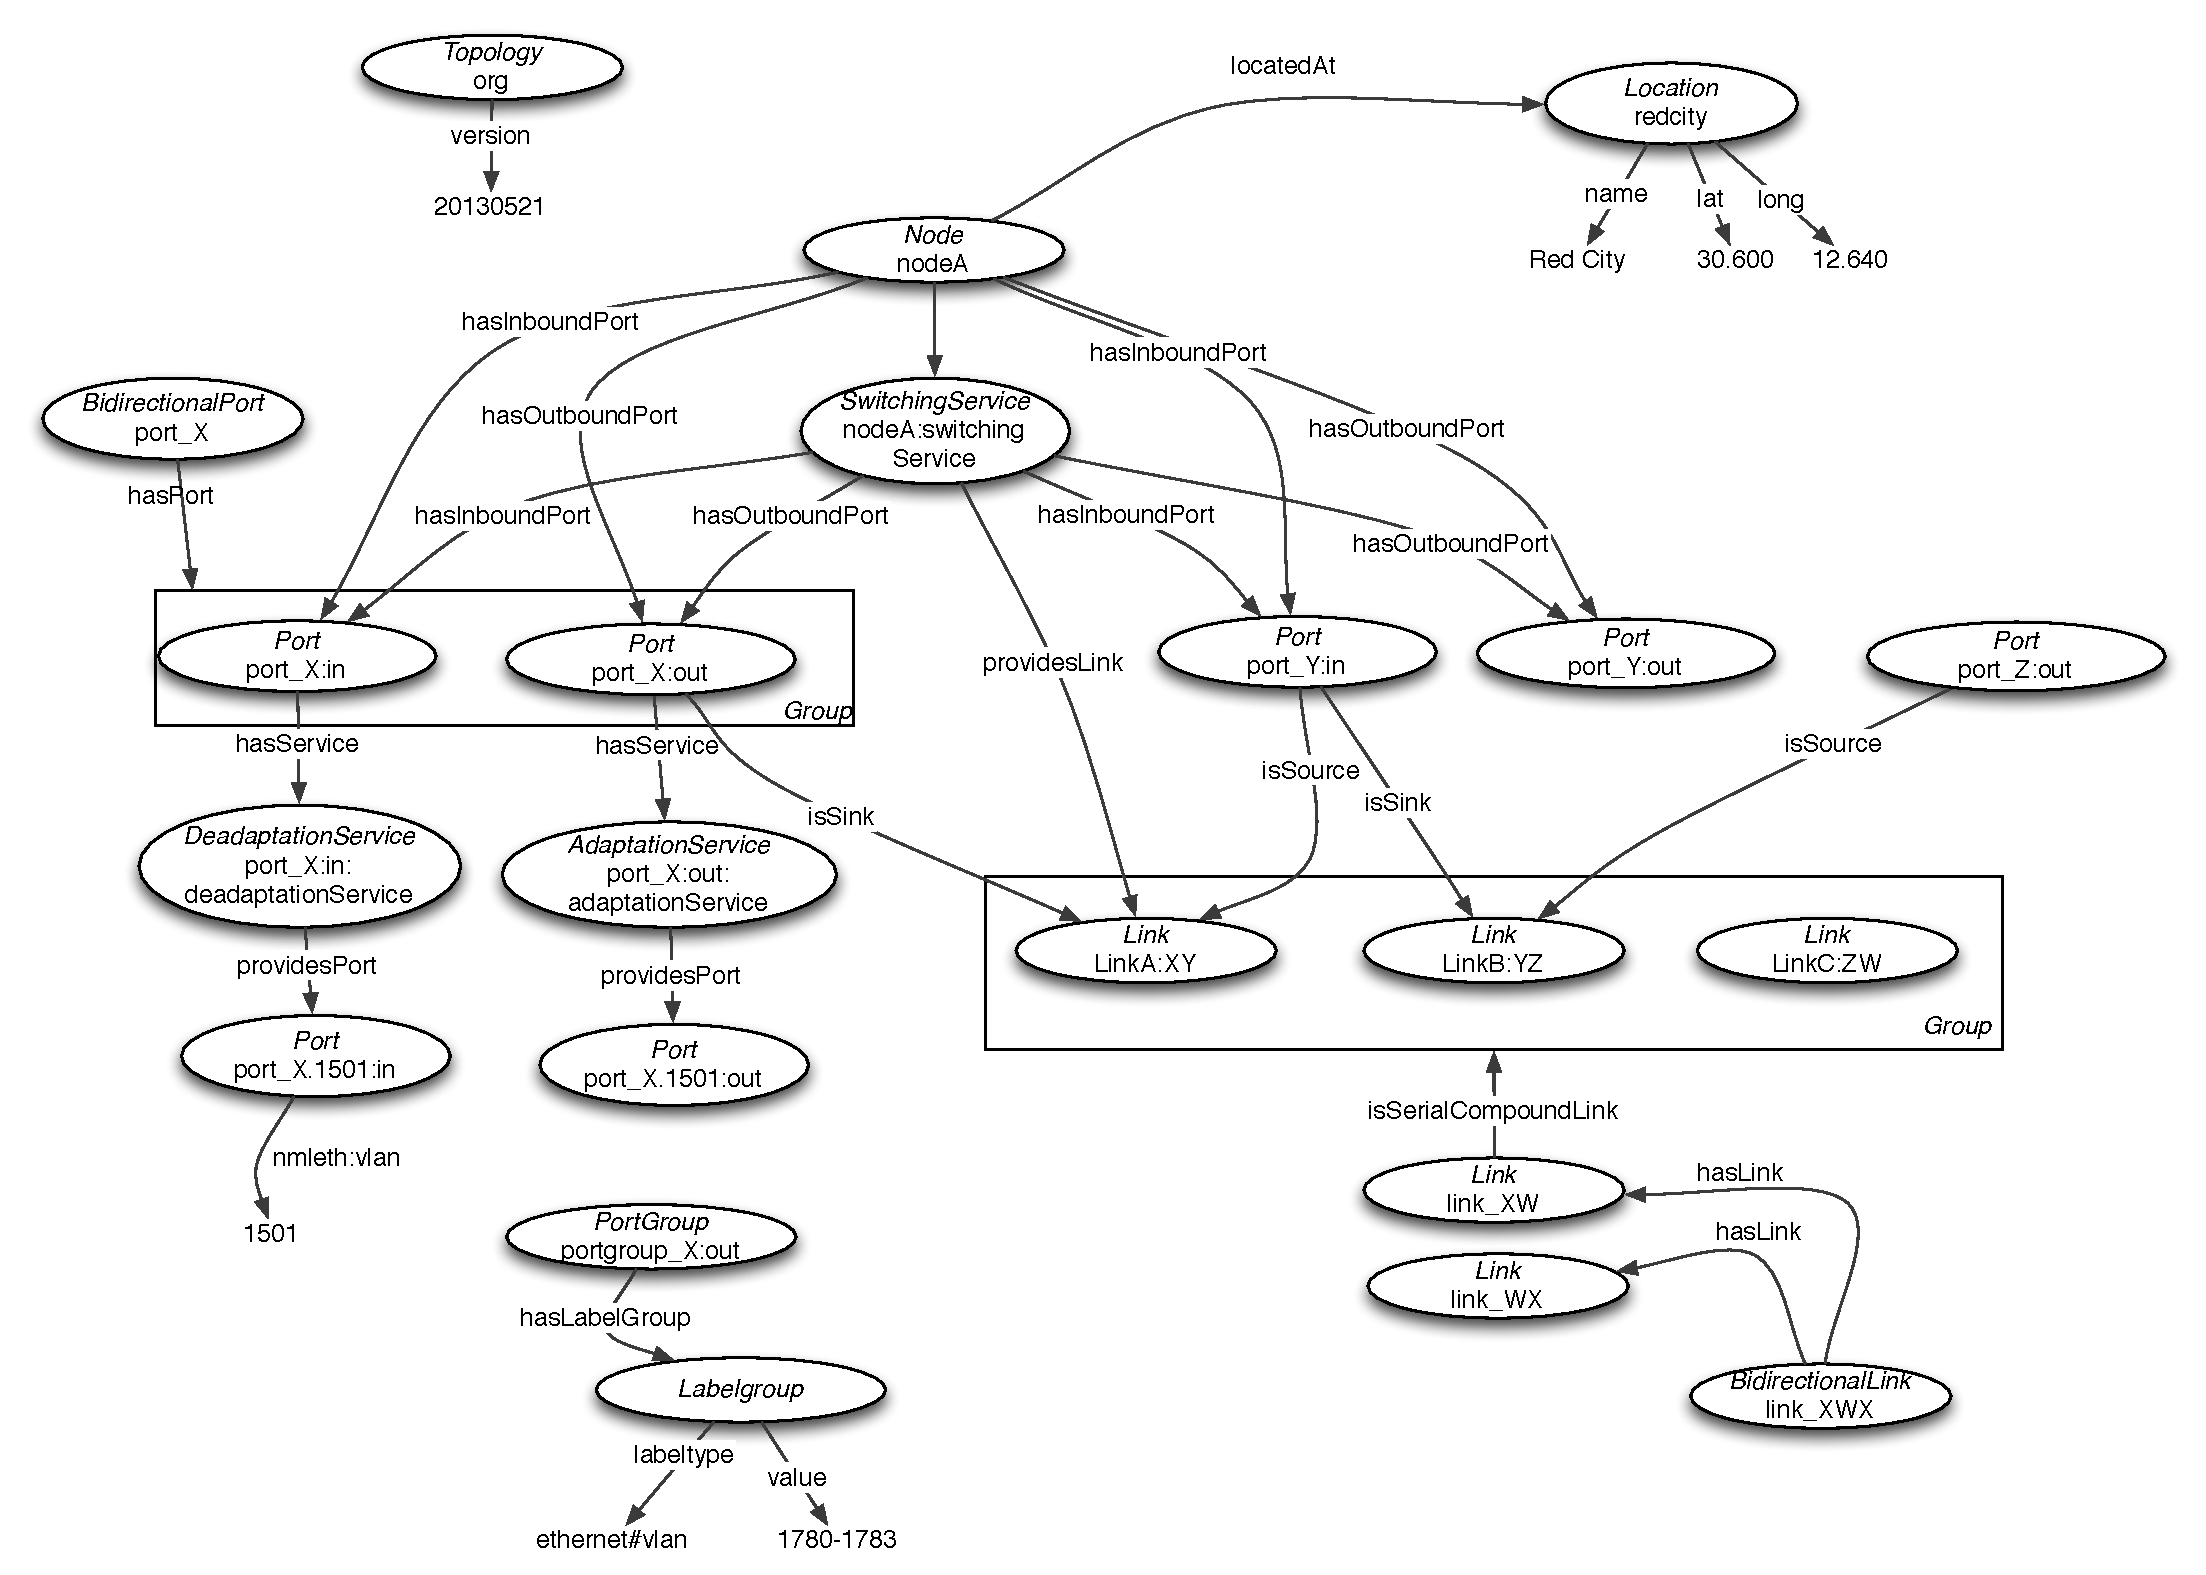
\includegraphics[width=\textwidth,angle=90]{combined-examples.pdf}
    \caption{A graphical overview showing the combination of all examples}
    \label{fig:combined-examples}
\end{figure}

\subsection{Examples in XML}
The following snippets represent NML structures in the XML format.

\begin{itemize}

    \item \emph{Topology} (section~\ref{class:topology})
      \lstinputlisting{xml/example-topology.xml}
    \item \emph{Node} (section~\ref{class:node})
      \lstinputlisting{xml/example-node.xml}
    \item \emph{Ports}  
      \begin{itemize}
        \item \emph{(Unidirectional) Port}  (section~\ref{class:port})
          \lstinputlisting{xml/example-port-unidir.xml}
        \item \emph{BidirectionalPort} (section~\ref{class:bidirectional_port})
          \lstinputlisting{xml/example-port-bidir.xml}
        \item \emph{PortGroup} (section~\ref{class:port_group})
          \lstinputlisting{xml/example-portgroup.xml}
      \end{itemize}
    \item \emph{Links} 
      \begin{itemize}
        \item \emph{UnidirectionalLink} (external) (section~\ref{class:link})
          \lstinputlisting{xml/example-link-unidir.xml}
        \item \emph{UnidirectionalLink} (internal) (section~\ref{class:link})
          \lstinputlisting{xml/example-link-unidir-cc.xml}
        \item \emph{UnidirectionalLink that is composed of more than one sub-link}
          \lstinputlisting{xml/example-link-serialcompound.xml}
        \item \emph{BidirectionalLink} (section~\ref{class:bidirectional_link})
          \lstinputlisting{xml/example-link-bidir.xml}
        \item \emph{LinkGroup} (section~\ref{class:link_group})
          \lstinputlisting{xml/example-linkgroup.xml}
      \end{itemize}
    \item \emph{Labels}
      \begin{itemize}
        \item \emph{Label} (section~\ref{class:label})
          \lstinputlisting{xml/example-label.xml}
        \item \emph{LabelGroup} (section~\ref{class:label_group})
          \lstinputlisting{xml/example-labelgroup.xml}
      \end{itemize}
    \item \emph{Location} (section~\ref{class:location})
      \lstinputlisting{xml/example-location.xml}
    \item \emph{Services}
      \begin{itemize}
        \item \emph{SwitchingService} (section~\ref{class:switching_service})
          \lstinputlisting{xml/example-switchingservice.xml}
        \item \emph{AdaptationService} (section~\ref{class:adaptation_service})
          \lstinputlisting{xml/example-adaptationservice.xml}
        \item \emph{DeadaptationService} (section~\ref{class:deadaptation_service})
          \lstinputlisting{xml/example-deadaptationservice.xml}
      \end{itemize}

\end{itemize}

\pagebreak

\subsection{Examples in OWL}
The following snippets represent NML structures in the OWL format.
The namespaces used in all the examples follow the definitions of the Topology example.

\begin{itemize}

    \item \emph{Topology} (section~\ref{class:topology})
      \lstinputlisting{owl/example-topology.xml}
    \item \emph{Node} (section~\ref{class:node})
      \lstinputlisting{owl/example-node.xml}
    \item \emph{Ports}  
      \begin{itemize}
        \item \emph{(Unidirectional) Port}  (section~\ref{class:port})
          \lstinputlisting{owl/example-port-unidir.xml}
        \item \emph{BidirectionalPort} (section~\ref{class:bidirectional_port})
          \lstinputlisting{owl/example-port-bidir.xml}
        \item \emph{PortGroup} (section~\ref{class:port_group})
          \lstinputlisting{owl/example-portgroup.xml}
      \end{itemize}
    \item \emph{Links} 
      \begin{itemize}
        \item \emph{UnidirectionalLink} (external) (section~\ref{class:link})
          \lstinputlisting{owl/example-link-unidir.xml}
        \item \emph{UnidirectionalLink} (internal) (section~\ref{class:link})
          \lstinputlisting{owl/example-link-unidir-cc.xml}
        \item \emph{UnidirectionalLink that is composed of more than one sub-link}
          \lstinputlisting{owl/example-link-serialcompound.xml}
        \item \emph{BidirectionalLink} (section~\ref{class:bidirectional_link})
          \lstinputlisting{owl/example-link-bidir.xml}
        \item \emph{LinkGroup} (section~\ref{class:link_group})
          \lstinputlisting{owl/example-linkgroup.xml}
      \end{itemize}
    \item \emph{Labels}
      \begin{itemize}
        \item \emph{Label} (section~\ref{class:label})
          \lstinputlisting{owl/example-label.xml}
        \item \emph{LabelGroup} (section~\ref{class:label_group})
          \lstinputlisting{owl/example-labelgroup.xml}
      \end{itemize}
    \item \emph{Location} (section~\ref{class:location})
      \lstinputlisting{owl/example-location.xml}
    \item \emph{Services}
      \begin{itemize}
        \item \emph{SwitchingService} (section~\ref{class:switching_service})
          \lstinputlisting{owl/example-switchingservice.xml}
        \item \emph{AdaptationService} (section~\ref{class:adaptation_service})
          \lstinputlisting{owl/example-adaptationservice.xml}
        \item \emph{DeadaptationService} (section~\ref{class:deadaptation_service})
          \lstinputlisting{owl/example-deadaptationservice.xml}
      \end{itemize}

\end{itemize}

\subsection{Conceptual Examples}

This section shows a few examples how NML was designed to be used. Like the other examples, this section is informative.  It may be possible that there are other ways to use the NML objects and attributes.

\subsubsection{Topology and Node}

A \emph{Topology} and \emph{Node} behave similar: they both contain inbound ports and outbound ports, and can contain a \emph{SwitchingService} to allow creation of internal links (cross connects) from inbound ports to outbound ports. Especially with the ability to create logical, sliced or virtual devices, the distinction is getting blurred.

The distinction is that a \emph{Node} is located at a single geographic location, while a \emph{Topology} is a set of geographically disperse Network Objects.

\subsubsection{Hierarchical Topology}

Large networks may want to publish both details of their network topology as a whole, as well as details about regional segments, without publishing details of the actual devices. NML allows the publication of a hierarchical \emph{Topology} tree, where the top-level \emph{Topology} has a \emph{hasTopology} relation with smaller \emph{Topologies}. These smaller Topologies must be fully enclosed -- the \emph{hasTopology} relation can not be used to relate partial overlapping Topologies.

For example, a \emph{Topology} \texttt{A} may want to publish about two parts of its Topology, \texttt{A\_West}, and \texttt{A\_East}. This allows it to publish difference in connectivity and costs between the two parts. It can do so with the following relations:

\nmlrelation{Topology \texttt{A}}{}{hasTopology}{}{Topology \texttt{A\_West}}\\
\nmlrelation{Topology \texttt{A}}{}{hasTopology}{}{Topology \texttt{A\_East}}

\subsubsection{Links, Segments and Paths}

A \emph{Link} object can refer to any link connection. A link segment and an end-to-end path are both described by a \emph{Link} object. This is by design, since it is easy to extend a \emph{Link}, or to describe a partition of a \emph{Link}.

Figure~\ref{fig:compound-link} gives an example of three different partitionings of a link between \texttt{port\_X:in} and \texttt{port\_W:out}.

\begin{figure}[htb]
    \centering
        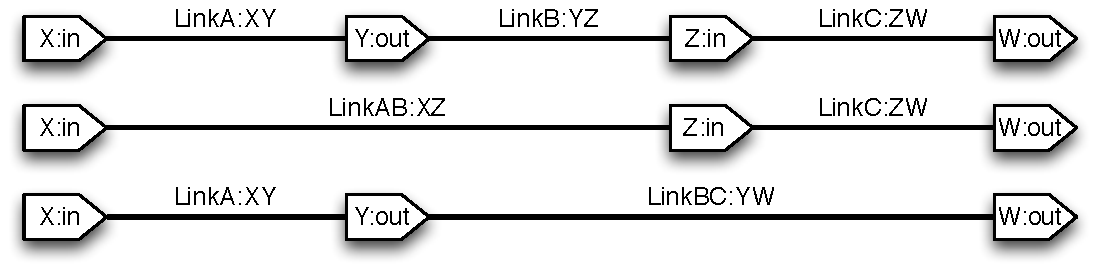
\includegraphics[width=.8\textwidth]{compound-link.pdf}
    \caption{Different partitionings of the same link.}
    \label{fig:compound-link}
\end{figure}

Note that in this example Port \texttt{port\_Y:out} is the source of both \texttt{linkB:YZ} and of \texttt{linkBC:YW}. If a single topology description would contain the full link and the partitioning, a path finding algoritm \MUST{} be aware that the fact that if a Port is the source of two NML Links, this does not mean it multicast to different network links. For this reason, it is \RECOMMENDED{} that applications either add metadata about the type of link, or specify that in certain messages, only one particular type of Link \MUST{} be used.


\subsubsection{Patch Panel and Media Convertor}

A port on a patch panel or optical distribution frame can simply be described as a NML Port (thus without an associated Node):

\nmlrelation{Port \texttt{odf\_X}}{}{isSink}{}{Link \texttt{A}}\\
\nmlrelation{Port \texttt{odf\_X}}{}{isSource}{}{Link \texttt{B}}

A mediaconvertor, e.g. from Ethernet over UTP to Ethernet over fiber, can be described in the same way, provided that the connected Links described the Ethernet connections. If the connected Links describe the underlying UTP and fiber connections, it is necessary to describe the conversion between them:

\nmlrelation{Port \texttt{Port\_X\_UTP}}{}{isSink}{}{Link \texttt{UTP\_A}} \\
\nmlrelation{Port \texttt{Port\_X\_fiber}}{}{isSource}{}{Link \texttt{fiber\_B}} \\
\nmlrelation{Port \texttt{Port\_X\_UTP}}{}{hasService}{}{DeAdaptataionService \texttt{X\_deadaptation}} \\
\nmlrelation{Port \texttt{Port\_X\_fiber}}{}{hasService}{}{AdaptationService \texttt{X\_adaptation}} \\
\nmlrelation{DeAdaptataionService \texttt{X\_deadaptation}}{}{providesPort}{}{Port \texttt{Port\_X\_eth}} \\
\nmlrelation{AdaptationService \texttt{X\_adaptation}}{}{providesPort}{}{Port \texttt{Port\_X\_eth}}


\subsubsection{VLAN and Broadcast Medium}

A VLAN is much like a broadcast medium, which can be described as a multipoint-to-multipoint Link:

\nmlrelation{Port \texttt{Port\_X:in}}{}{isSink}{}{Link \texttt{VLAN\_42}} \\
\nmlrelation{Port \texttt{Port\_X:out}}{}{isSink}{}{Link \texttt{VLAN\_42}} \\
\nmlrelation{Port \texttt{Port\_Y:in}}{}{isSink}{}{Link \texttt{VLAN\_42}} \\
\nmlrelation{Port \texttt{Port\_Y:out}}{}{isSink}{}{Link \texttt{VLAN\_42}} \\
\nmlrelation{Port \texttt{Port\_Z:in}}{}{isSink}{}{Link \texttt{VLAN\_42}} \\
\nmlrelation{Port \texttt{Port\_Z:out}}{}{isSink}{}{Link \texttt{VLAN\_42}} \\

Where \texttt{X}, \texttt{Y} and \texttt{Z} are in fact bidirectional ports:

\nmlrelation{BidirectionalPort \texttt{Port\_X}}{}{hasPort}{}{Port \texttt{Port\_X:in}} \\
\nmlrelation{BidirectionalPort \texttt{Port\_X}}{}{hasPort}{}{Port \texttt{Port\_X:out}} \\
\nmlrelation{BidirectionalPort \texttt{Port\_Y}}{}{hasPort}{}{Port \texttt{Port\_Y:in}} \\
\nmlrelation{BidirectionalPort \texttt{Port\_Y}}{}{hasPort}{}{Port \texttt{Port\_Y:out}} \\
\nmlrelation{BidirectionalPort \texttt{Port\_Z}}{}{hasPort}{}{Port \texttt{Port\_Z:in}} \\
\nmlrelation{BidirectionalPort \texttt{Port\_Z}}{}{hasPort}{}{Port \texttt{Port\_Z:out}} \\

However, this is not entirely correct: in the above description data coming from \texttt{Port\_X:in} would also be forwarded to \texttt{Port\_X:out}. However, the Ethernet technology prevents data returning on the same interface.

NML introduced the \emph{noReturnTraffic} parameter to describe this technological restriction: if the \emph{noReturnTraffic} parameter of a Link is true, there is no data transport from a source to a sink if the source and sink are grouped together in a BidirectionalPort group.

\nmlrelation{Link VLAN\_42}{}{noReturnTraffic}{}{"\texttt{true}"} \\


\subsubsection{Configuration and Potential Capability}

NML is able to both describe the network services (potential capability) as well as the network configuration.

A switching service can be described by a SwitchingService object along with associated inbound ports and outbound ports:

\nmlrelation{SwitchingService \texttt{switchmatrix\_A}}{}{hasInboundPort}{}{PortGroup \texttt{Port\_X:in}} \\
\nmlrelation{SwitchingService \texttt{switchmatrix\_A}}{}{hasOutboundPort}{}{PortGroup \texttt{Port\_X:out}} \\
\nmlrelation{SwitchingService \texttt{switchmatrix\_A}}{}{hasInboundPort}{}{PortGroup \texttt{Port\_Y:in}} \\
\nmlrelation{SwitchingService \texttt{switchmatrix\_A}}{}{hasOutboundPort}{}{PortGroup \texttt{Port\_Y:out}} \\
\nmlrelation{SwitchingService \texttt{switchmatrix\_A}}{}{labelSwapping}{}{\texttt{true}}

A cross connect created by this switching service can be specified by a Link object:

\nmlrelation{SwitchingService \texttt{switchmatrix\_A}}{}{providesLink}{}{Link \texttt{crossconnect\_A.1501}} \\
\nmlrelation{PortGroup \texttt{Port\_X:in}}{}{hasPort}{}{Port \texttt{Port\_X.1501:in}} \\
\nmlrelation{PortGroup \texttt{Port\_Y:out}}{}{hasPort}{}{Port \texttt{Port\_Y.1501:out}} \\
\nmlrelation{Port \texttt{Port\_X.1501:in}}{}{isSource}{}{Link \texttt{crossconnect\_A.1501}} \\
\nmlrelation{Port \texttt{Port\_Y.1501:out}}{}{isSink}{}{Link \texttt{crossconnect\_A.1501}}

An encoding and decoding service can be described by a AdapdationService and DeAdaptationService:

\nmlrelation{Port \texttt{Port\_X\_fiber:in}}{}{hasService}{}{DeAdaptationService \texttt{port\_X:in:deadaptation}} \\
\nmlrelation{DeAdaptationService \texttt{port\_X:in:deadaptation}}{}{canProvidePort}{}{PortGroup \texttt{Port\_X:in}}

A channel created by this encoding service can be specified by a \emph{providesPort} relation:

\nmlrelation{DeAdaptationService \texttt{port\_X:in:deadaptation}}{}{providesPort}{}{Port \texttt{Port\_X.1501:in}} \\
\nmlrelation{PortGroup \texttt{Port\_X:in}}{}{hasPort}{}{Port \texttt{Port\_X.1501:in}}


\subsubsection{Versioning and Lifetime}

The version of a \emph{Topology} indicated the serial number. If there are two \emph{Topology} descriptions for the same network, the one with the highest version number is the most recent version. The \emph{LifeTime} object is used to indicate when a certain resource is available.

Imagine that a link will have a scheduled downtime due to maintenance next week between 2 AM and 4 AM. This can be specified with these relations:

\nmlrelation{Topology \texttt{org}}{}{version}{}{\texttt{20130521T000000Z}} \\
\nmlrelation{Link \texttt{A}}{}{existsDuring}{}{LifeTime \texttt{A\_lifetime1}} \\
\nmlrelation{Link \texttt{A}}{}{existsDuring}{}{LifeTime \texttt{A\_lifetime2}} \\
\nmlrelation{LifeTime \texttt{A\_lifetime1}}{}{end}{}{\texttt{20130611T020000Z}} \\
\nmlrelation{LifeTime \texttt{A\_lifetime2}}{}{start}{}{\texttt{20130611T040000Z}}

Imagine that this planned maintainance is rescheduled. That can be specified by creating a new Topology with a new version number, and updated data:

\nmlrelation{Topology \texttt{org}}{}{version}{}{\texttt{20130604T000000Z}} \\
\nmlrelation{Link \texttt{A}}{}{existsDuring}{}{LifeTime \texttt{A\_lifetime1}} \\
\nmlrelation{Link \texttt{A}}{}{existsDuring}{}{LifeTime \texttt{A\_lifetime2}} \\
\nmlrelation{LifeTime \texttt{A\_lifetime1}}{}{end}{}{\texttt{20130618T020000Z}} \\
\nmlrelation{LifeTime \texttt{A\_lifetime2}}{}{start}{}{\texttt{20130618T040000Z}}



\newpage
%!TEX root = nml-base.tex

\section{NML Base Schema}%
\label{s:schema}

The NML Base schema describes an information model for computer networks. 
This schema is kept intentionally general, with provisions to extend the schema to 
describe layer-specific information.

The schema consists of classes, attributes, relations, and parameters. % and logic. 
Classes describe types of objects and are described in section~\ref{sub:classes}. 
Relations describe the relations between classes and are described in section~\ref{sub:relations}. 
Attributes describe properties of classes.
% Logic describes how some relations may be derived from other relations.
Parameters, like attributes, are properties of classes, but may (subtly) change the logic.
% Logic is described in section~\ref{sub:logic}.
Attributes and parameters are described with their class description.

All classes, relations, attributes and parameters defined in this document have an 
identifier within the namespace \texttt{http://schemas.ogf.org/nml/2013/05/base\#}.

\subsection{Classes}%
\label{sub:classes}

\begin{figure}[!b]
    \centering
        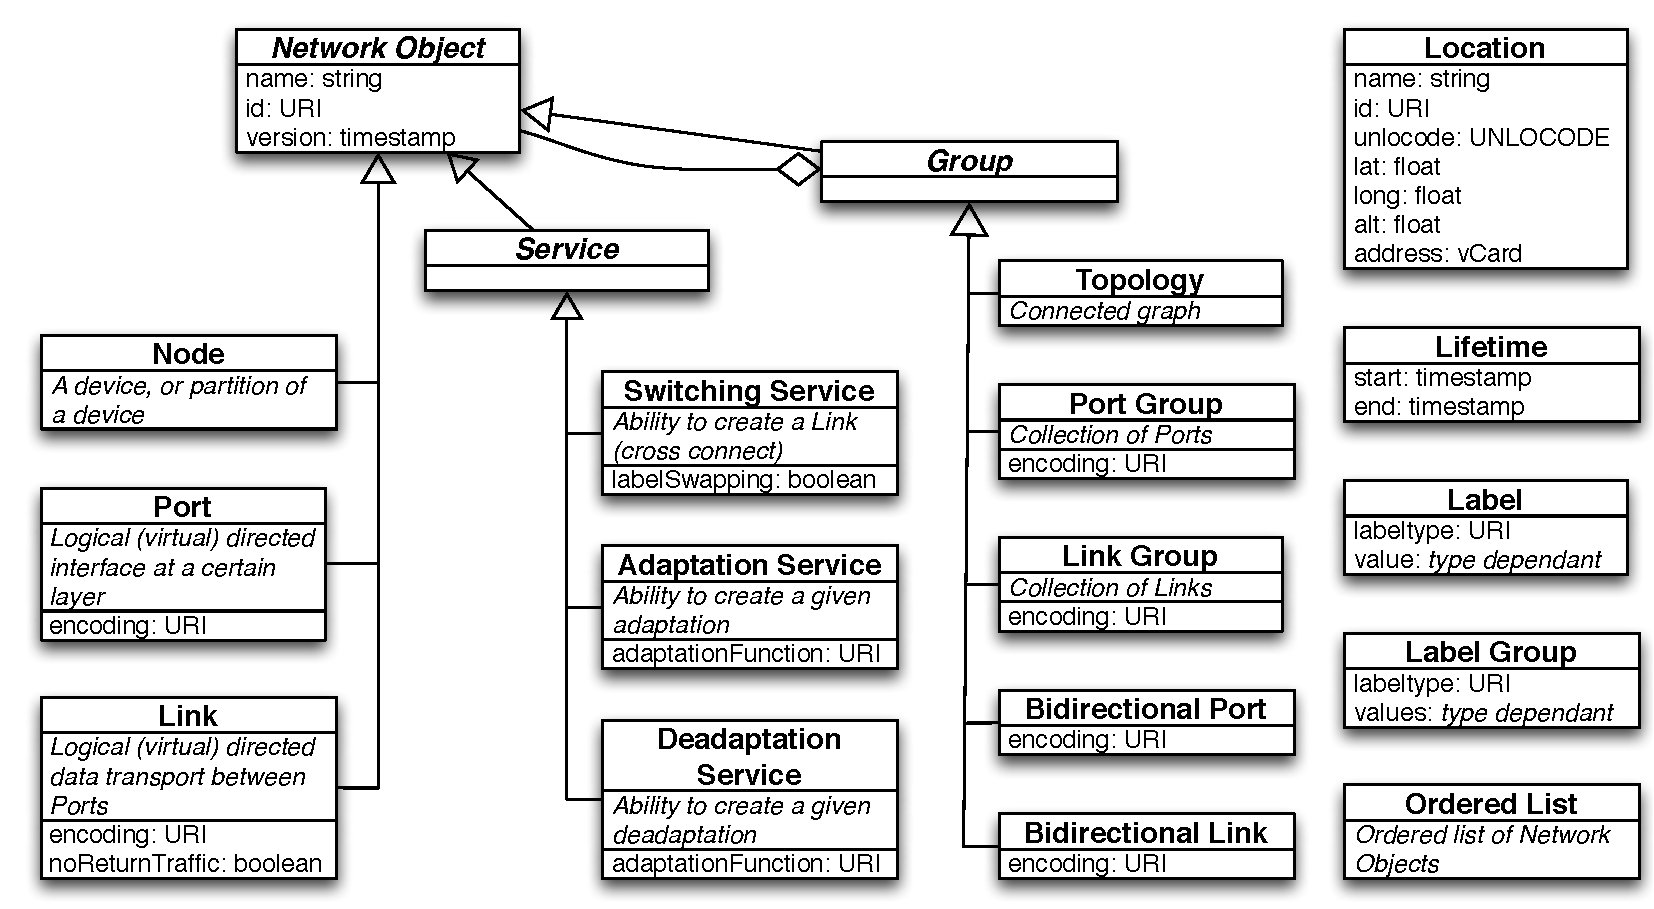
\includegraphics[width=\textwidth]{NML-hierarchy}
    \caption{A UML class diagram of the classes in the NML schema and their hierarchy}
    \label{fig:NML-schema}
\end{figure}

Figure~\ref{fig:NML-schema} shows an overview of all the classes in the NML schema in a UML class diagram. Each box defines the name of a class, a short description, and possible attributes with their value type.
%The figure also shows the relations between the objects, and their cardinalities. 
In the sections below we discuss each of the elements of the schema.

\subsubsection{Network Object}% (fold)
\label{class:network_object}

The basic abstract class of the schema is the \emph{Network Object}.  Most classes inherit from it.

\emph{Network Object} is an abstract class. It \MUSTNOT{} be instantiated directly.

A \emph{Network Object} may have the following relations:
\begin{itemize}
    \item \emph{existsDuring} to one or more \emph{Lifetime}s
    \item \emph{isAlias} to one or more \emph{Network Object}s
    \item \emph{locatedAt} to one \emph{Location} 
\end{itemize}

A \emph{Network Object} may have the following attributes:
\begin{itemize}
    \item \emph{id} to assign a persistent globally unique URI
    \item \emph{name} to assign a human readable string
    \item \emph{version} to assign a time stamp
\end{itemize}

The meaning of the \emph{isAlias} relation is only defined for specific cases (between objects of the same concrete class), and \SHOULDNOT{} be used between other objects.

The meaning of the \emph{version} attribute is only defined for specific cases (for objects of the Topology class), and \SHOULDNOT{} be used in other objects. Clients that receive a \emph{version} attribute for a non-\emph{Topology} object \SHOULD{} ignore that attribute.

An \emph{id} is a persistent, globally unique object identifier for the \emph{Network Object}. The \emph{id} \SHOULD{} be used to refer to this object. Section~\ref{s:identifiers} describes these identifiers in detail.

\emph{name} is a human readable string.
A name may be written in any language, but it is \RECOMMENDED{} that names are chosen so that all users can easily distinguish between different names. Names are not globally unique, and two objects can have the same name. It is \RECOMMENDED{} to use short, descriptive names.
A name \MUSTNOT{} be used for anything other than display purposes.  Normal Unicode recommendations apply: A name \MUSTNOT{} contain control or formatting codepoint, and it is \RECOMMENDED{} to only use codepoints from the Basic Multilingual Plane (BMP).

\emph{version} is a time stamp formatted as ISO 8601 calendar date, and \MUST{} be a basic (compact) representation with UTC timezone (\texttt{\emph{YYYYMMDD}T\emph{hhmmss}Z})~\cite{iso8601}. The time stamp can be used to publish updates of a \emph{Topology}. 
If a client receives multiple \emph{Topology} descriptions, each with a different version time stamp, the version with the latest time stamp in the past or present \MUST{} be considered the valid description. \emph{Topology} descriptions with a time stamp in the future \MAY{} be discarded or cached until the denoted time. See also the \emph{Lifetime} object to describe historic or future network changes.

The base \emph{Network Object} is subclassed into the top-level topology
components, that are sufficient to cover the description of networks.  The
classes in this schema that directly inherit from \emph{Network Object} are:

\begin{itemize}
    \item Node
    \item Port
    \item Link
    \item Service
    \item Group
\end{itemize}

These classes are described in more detail below.
% subsection network_object (end)


\subsubsection{Node}% (fold)
\label{class:node}

A \emph{Node} is generally a device connected to, or part of, the network.  A
Node does not necessarily correspond to a physical machine.

\emph{Node} inherits from \emph{Network Object}.

A \emph{Node} may have the following relations:
\begin{itemize}
    \item \emph{existsDuring} to one or more \emph{Lifetime}s
    \item \emph{hasInboundPort} to one or more \emph{Port}s or \emph{PortGroup}s
    \item \emph{hasOutboundPort} to one or more \emph{Port}s or \emph{PortGroup}s
    \item \emph{hasService} to one or more \emph{Service}s of type \emph{Switch}
    \item \emph{implementedBy} to one or more \emph{Node}s
    \item \emph{isAlias} to one or more \emph{Node}s
    \item \emph{locatedAt} to one \emph{Location} 
\end{itemize}

A \emph{Node} may have the following attributes:
\begin{itemize}
    \item \emph{id} to assign a persistent globally unique URI
    \item \emph{name} to assign a human readable string
\end{itemize}

% subsection node (end)


\subsubsection{Port}% (fold)
\label{class:port}

A \emph{Port} defines connectivity from a \emph{Network Object} to the rest of the network. A \emph{Port} object is unidirectional. A \emph{Port} does not necessarily correspond to a physical interface. It represents a logical transport entity at a fixed place in the network.

\emph{Port} inherits from \emph{Network Object}.

A \emph{Port} may have the following relations:
\begin{itemize}
    \item \emph{existsDuring} to one or more \emph{Lifetime}s
    \item \emph{hasLabel} to one \emph{Label}
    \item \emph{hasService} to one or more \emph{Service}s of type \emph{Adaptation} or type \emph{Deadaptation}
    \item \emph{isAlias} to one or more \emph{Port}s
    \item \emph{isSink} to one or more \emph{Link}s
    \item \emph{isSource} to one or more \emph{Link}s
\end{itemize}

A \emph{Port} may have the following attributes:
\begin{itemize}
    \item \emph{encoding} to assign a data encoding identifier
    \item \emph{id} to assign a persistent globally unique URI
    \item \emph{name} to assign a human readable string
\end{itemize}

The \emph{encoding} attribute defines the format of the data streaming through the Port. The identifier for the encoding \MUST{} be a URI. Encoding URIs \SHOULD{} be specified in a Grid Forum Documents (GFD).
% subsection port (end)


\subsubsection{Link}% (fold)
\label{class:link}

A \emph{Link} object describes a unidirectional data transport from each of its sources to all of its sinks.

A source of a Link is a Network Object, e.g.\ a \emph{Port}, that has a \emph{isSource} relation to the \emph{Link}.
A sink of a Link is a Network Object, e.g.\ a \emph{Port}, that has a \emph{isSink} relation to the \emph{Link}.

A \emph{Link} object can refer to any link connection. A link segment and an end-to-end path are both described by a \emph{Link} object. The composition of links into a path, and decomposition into link segments is described by the \emph{isSerialCompoundLink} relation.

\emph{Link} inherits from \emph{Network Object}.

A \emph{Link} may have the following relations:
\begin{itemize}
    \item \emph{existsDuring} to one or more \emph{Lifetime}s
    \item \emph{hasLabel} to one \emph{Label}
    \item \emph{isAlias} to one or more \emph{Link}s
    \item \emph{isSerialCompoundLink} to one \emph{Ordered List} of \emph{Link}s
\end{itemize}

A \emph{Link} may have the following attributes:
\begin{itemize}
    \item \emph{encoding} to assign a data encoding identifier
    \item \emph{id} to assign a persistent globally unique URI
    \item \emph{name} to assign a human readable string
\end{itemize}

A \emph{Link} may have the following parameter:
\begin{itemize}
    \item \emph{noReturnTraffic}. A value of \texttt{true} changes the definition of \emph{Link} to: data transport from each sources to all sinks, except that there is no data transport from a source to a sink if the source and sink are grouped together in a \emph{BidirectionalPort} group. The default value of \emph{noReturnTraffic} is \texttt{false}.
    
    An example of where this is used is in an Ethernet broadcast domain, where broadcast traffic is sent to all sinks, except the sink \emph{Port}s associated with the sending source \emph{Port}.
\end{itemize}

The \emph{encoding} attribute defines the format of the data streaming through the \emph{Link}. The identifier for the encoding \MUST{} be a URI. Encoding URIs \SHOULD{} be specified in a Grid Forum Documents (GFD).
% subsection link (end)


\subsubsection{Service}% (fold)
\label{class:service}

\emph{Service} describes an ability of the network. That is, it describes how the behavior can be changed dynamically.

\emph{Service} is an abstract class. It \MUSTNOT{} be instantiated directly.

\emph{Service} inherits from \emph{Network Object}.
A \emph{Service} may have the same relations, attributes and parameters as a \emph{Network Object}.

This schema defines three different services, the \emph{SwitchingService} the \emph{AdaptationService} and the \emph{DeadaptationService}. These are described in more detail below. 
% subsection service (end)


\subsubsection{Switching Service}% (fold)
\label{class:switching_service}

A \emph{SwitchingService} describes the ability to create new \emph{Link}s from any of its inbound \emph{Port}s to any of its outbound \emph{Port}s.

\emph{SwitchingService} inherits from \emph{Service}.

A \emph{SwitchingService} may have the following relations:
\begin{itemize}
    \item \emph{encoding} to assign a data encoding identifier
    \item \emph{existsDuring} to one or more \emph{Lifetime}s
    \item \emph{hasInboundPort} to one or more \emph{Port}s or \emph{PortGroup}s
    \item \emph{hasOutboundPort} to one or more \emph{Port}s or \emph{PortGroup}s
    \item \emph{isAlias} to one or more \emph{Switching Service}s
    \item \emph{providesLink} to one or more \emph{Link}s or \emph{LinkGroup}s.
\end{itemize}

A \emph{SwitchingService} may have the following attributes:
\begin{itemize}
    \item \emph{id} to assign a persistent globally unique URI
    \item \emph{name} to assign a human readable string
\end{itemize}

A \emph{SwitchingService} may have the following parameter:
\begin{itemize}
    \item \emph{labelSwapping}. A value of \texttt{false} adds a restriction to the \emph{SwitchingService}: it is only able to create cross connects from an inbound \emph{Port} to an outbound \emph{Port} if the \emph{Label} of the connected \emph{Port}s have the same value. The default value is \texttt{false}.
\end{itemize}

The \emph{providesLink} relation points to \emph{Link}s which describe the currently configured cross connects in a \emph{SwitchingService}.

A \emph{Port} object can have a \emph{hasService} relation, however the \emph{SwitchingService} defines a more specific relation \emph{hasInboundPort} / \emph{hasOutboundPort} relation to a \emph{Port} object. The latter relation is preferred over the \emph{hasService} relation of the Port to the SwitchingService.

The \emph{encoding} attribute defines the format of the data streaming through the \emph{SwitchingService}. The identifier for the encoding \MUST{} be a URI. Encoding URIs \SHOULD{} be specified in a Grid Forum Documents (GFD).
% subsection switching_service (end)


\subsubsection{Adaptation Service}% (fold)
\label{class:adaptation_service}

An \emph{AdaptationService} describes the ability that data from one or more \emph{Port}s can be embedded in the data encoding of one other \emph{Port}. This is commonly referred to as the embedding of client layer (higher network layer) ports in a server layer (lower network layer) port. The \emph{AdaptationService} describes a multiplexing adaptation function, meaning that different channels (the client layer ports) can be embedded in a single data stream (the server layer port). For example multiplexing several VLANs over a single trunk port.

Like \emph{Port} and \emph{Link}, \emph{AdaptationService} describes a unidirectional transport function. For the inverse transport function, see \emph{DeadaptationService}.

\emph{AdaptationService} inherits from \emph{Service}.

An \emph{AdaptationService} may have the following relations:
\begin{itemize}
    \item \emph{canProvidePort} to one or more \emph{Port}s or \emph{PortGroup}s (this describes a ability)
    \item \emph{existsDuring} to one or more \emph{Lifetime}s
    \item \emph{isAlias} to one or more \emph{AdaptationService}s
    \item \emph{providesPort} to one or more \emph{Port}s or \emph{PortGroup}s (this describes a configuration)
\end{itemize}

An \emph{AdaptationService} may have the following attributes:
\begin{itemize}
    \item \emph{adaptationFunction} to assign an adaptation technology identifier
    \item \emph{id} to assign a persistent globally unique URI
    \item \emph{name} to assign a human readable string
\end{itemize}

\emph{DeadaptationService} is an inverse of \emph{AdaptationService}. This should not be confused with an inverse multiplexing adaptation function. An inverse multiplexing adaptation function embeds a single data stream in multiple underlying data streams. To describes such a network, the \emph{parallelCompound} relation can be used, which is a future extension relation, described in a separate document~\cite{nml-experimental}.

% subsection adaptation_service (end)


\subsubsection{De-adaptation Service}% (fold)
\label{class:deadaptation_service}

A \emph{DeadaptationService} describes the ability that data of one or more ports can be extracted from the data encoding of one other port. This is commonly referred to as the extraction of client layer (higher network layer) ports from the server layer (lower network layer) port. The \emph{DeadaptationService} describes a demultiplexing adaptation function, meaning that different channels (the client layer ports) can be extracted from a single data stream (the server layer port). For example demultiplexing several VLANs from a single trunk port.

Like \emph{Port} and \emph{Link}, \emph{AdaptationService} describes a unidirectional transport function. For the inverse transport function, see \emph{AdaptationService}.%

\emph{DeadaptationService} inherits from \emph{Service}.

A \emph{DeadaptationService} may have the following relations:
\begin{itemize}
    \item \emph{canProvidePort} to one or more \emph{Port}s or \emph{PortGroup}s
    \item \emph{existsDuring} to one or more \emph{Lifetime}s
    \item \emph{isAlias} to one or more \emph{DeadaptationService}s
    \item \emph{providesPort} to one or more \emph{Port}s or \emph{PortGroup}s
\end{itemize}

A \emph{DeadaptationService} may have the following attributes:
\begin{itemize}
    \item \emph{adaptationFunction} to assign a adaptation technology identifier
    \item \emph{id} to assign a persistent globally unique URI
    \item \emph{name} to assign a human readable string
\end{itemize}

% subsubsection adaptation_service (end)


\subsubsection{Group}% (fold)
\label{class:group}

A \emph{Group} describes a collections of objects. Any object can be part of a group, including another \emph{Group}. An object can also be part of multiple \emph{Group}s.

\emph{Group} is an abstract class. It \MUSTNOT{} be instantiated directly.

\emph{Group} inherits from \emph{Network Object}.
A \emph{Group} may have the same relations, attributes and parameters as a \emph{Network Object}.

This schema defines five different \emph{Group}s:

\begin{itemize}
    \item Topology
    \item Port Group
    \item Link Group
    \item Bidirectional Port
    \item Bidirectional Link
\end{itemize}

These classes are described in more detail below.
% subsubsection group (end)



\subsubsection{Topology}% (fold)
\label{class:topology}

A \emph{Topology}\footnote{At first this was called a Network, then Graph Network. The term Topology was suggested to avoid the confusion surrounding the overloaded term Network.} is a set of connected \emph{Network Object}s. \emph{connected} means that there is, or it is possible to create, a data transport between any two Network Objects in the same Topology, provided that there are no policy, availability or technical restrictions.

A \emph{Topology} may have the following relations:
\begin{itemize}
    \item \emph{existsDuring} to one or more \emph{Lifetime}s
    \item \emph{hasNode} to one or more \emph{Node}s
    \item \emph{hasInboundPort} to one or more \emph{Port}s or \emph{PortGroup}s
    \item \emph{hasOutboundPort} to one or more \emph{Port}s or \emph{PortGroup}s
    \item \emph{hasService} to one or more \emph{Service} of type \emph{Switch}
    \item \emph{hasTopology} to one or more \emph{Topology}s
    \item \emph{isAlias} to one or more \emph{Topology}s
    \item \emph{locatedAt} to one \emph{Location} 
\end{itemize}

A \emph{Topology} may have the following attributes:
\begin{itemize}
    \item \emph{id} to assign a persistent globally unique URI
    \item \emph{name} to assign a human readable string
    \item \emph{version} to assign a serial number
\end{itemize}

The \emph{version} attribute is described at the \emph{Network Object}.
% subsubsection topology (end)


\subsubsection{Port Group}% (fold)
\label{class:port_group}

A \emph{PortGroup} is an unordered set of \emph{Port}s.

A \emph{PortGroup} may have the following relations:
\begin{itemize}
    \item \emph{existsDuring} to one or more \emph{Lifetime}s
    \item \emph{hasLabelGroup} to one \emph{LabelGroup}
    \item \emph{hasPort} to one or more \emph{Port}s or \emph{PortGroups}
    % \item \emph{hasService} to one or more \emph{Service}s of type Adaptation or type Deadaptation
    \item \emph{isAlias} to one or more \emph{PortGroup}s
    \item \emph{isSink} to one or more \emph{LinkGroup}s
    \item \emph{isSource} to one or more \emph{LinkGroup}s
\end{itemize}

A \emph{PortGroup} may have the following attributes:
\begin{itemize}
    \item \emph{encoding} to assign a data encoding identifier
    \item \emph{id} to assign a persistent globally unique URI
    \item \emph{name} to assign a human readable string
\end{itemize}

% subsubsection port_group (end)


\subsubsection{Link Group}% (fold)
\label{class:link_group}

A \emph{LinkGroup} is an unordered set of \emph{Link}s.

A \emph{LinkGroup} may have the following relations:
\begin{itemize}
    \item \emph{existsDuring} to one or more \emph{Lifetime}s
    \item \emph{hasLabelGroup} to one \emph{LabelGroup}
    \item \emph{hasLink} to one or more \emph{Link}s or \emph{LinkGroup}s
    \item \emph{isAlias} to one or more \emph{LinkGroup}s
    \item \emph{isSerialCompoundLink} to \emph{Ordered List} of \emph{LinkGroup}s
\end{itemize}

A \emph{LinkGroup} may have the following attributes:
\begin{itemize}
    \item \emph{id} to assign a persistent globally unique URI
    \item \emph{name} to assign a human readable string
\end{itemize}

% subsubsection link_group (end)


\subsubsection{Bidirectional Port}% (fold)
\label{class:bidirectional_port}

A \emph{BidirectionalPort} is a group of two (unidirectional) 
\emph{Port}s or \emph{PortGroup}s together forming a bidirectional representation of a physical or 
virtual port. See Figure~\ref{fig:Port-Link} for an example of a \emph{BidirectionalPort} and its associated \emph{Port}s.

A \emph{BidirectionalPort} may have the following relations:
\begin{itemize}
    \item \emph{existsDuring} to one or more \emph{Lifetime}s
    \item \emph{hasPort} to exactly two \emph{Port}s or two \emph{PortGroup}s
\end{itemize}

A \emph{BidirectionalPort} may have the following attributes:
\begin{itemize}
    \item \emph{encoding} to assign a data encoding identifier
    \item \emph{id} to assign a persistent globally unique URI
    \item \emph{name} to assign a human readable string
\end{itemize}

There is explicitly no direct relation between a \emph{BidirectionalPort} and a \emph{BidirectionalLink}, since NML is a unidirectional model.
% subsubsection bidirectional_port (end)

\begin{figure}[htbp]
    \centering
        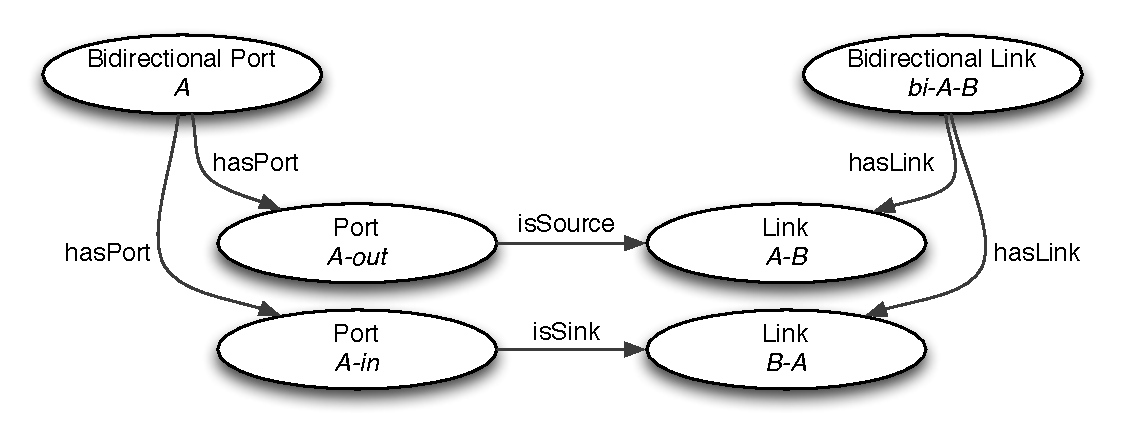
\includegraphics[width=.8\textwidth]{Port-Link.pdf}
    \caption{An abstract example of \emph{BidirectionalPort} and \emph{BidirectionalLink}}
    \label{fig:Port-Link}
\end{figure}


\subsubsection{Bidirectional Link}% (fold)
\label{class:bidirectional_link}

A \emph{BidirectionalLink} is a group of two (unidirectional) \emph{Link}s or \emph{LinkGroup}s together forming a bidirectional link. See Figure~\ref{fig:Port-Link} for an example of a \emph{BidirectionalLink} and its associated \emph{Link}s.

A \emph{BidirectionalLink} may have the following relations:
\begin{itemize}
    \item \emph{existsDuring} to one or more \emph{Lifetime}s
    \item \emph{hasLink} to exactly two \emph{Link}s or two \emph{LinkGroup}s
\end{itemize}

A \emph{BidirectionalLink} may have the following attributes:
\begin{itemize}
    \item \emph{encoding} to assign a data encoding identifier
    \item \emph{id} to assign a persistent globally unique URI
    \item \emph{name} to assign a human readable string
\end{itemize}

There is explicitly no direct relation between a \emph{BidirectionalPort} and a \emph{BidirectionalLink}, since NML is a unidirectional model.
% subsubsection bidirectional_link (end)


\subsubsection{Location}% (fold)
\label{class:location}

A \emph{Location} is a reference to a geographical location or area. A \emph{Location} object can be related to other \emph{Network Object}s to describe that these are located there. This can be relevant for network measurements, visualisations, et cetera.

A \emph{Location} may have the following attributes:
\begin{itemize}
    \item \emph{id} to assign a persistent globally unique URI
    \item \emph{name} to assign a human readable string
    \item \emph{long} is the longitude in WGS84 coordinate system (in decimal degrees)~\cite{wgs84}
    \item \emph{lat} is the latitude in WGS84 coordinate system (in decimal degrees)
    \item \emph{alt} is the altitude in WGS84 coordinate system (in decimal meters) 
    \item \emph{unlocode} is the UN/LOCODE location identifier~\cite{unlocode}
    \item \emph{address} is a vCard ADR (address) property. The exact syntax of the address property is not specified, to allow other (e.g.\ XML or RDF) representations of the string-based format specified in \cite{vcard}.
\end{itemize}

% subsubsection location (end)


\subsubsection{Lifetime}% (fold)
\label{class:lifetime}

A \emph{Lifetime} is an interval between which the object is said to be active. This can be used to track changes in a network, reflect dynamic operations, to help debug problems, et cetera.

A \emph{Lifetime} \MAY{} have the following attributes:
\begin{itemize}
    \item \emph{start} is the start time and date formatted as ISO 8601 calendar date, and \SHOULD{} be a basic (compact) representation with UTC timezone (\texttt{\emph{YYYYMMDD}T\emph{hhmmss}Z})~\cite{iso8601}
    \item \emph{end} is the end time and date formatted as ISO 8601 calendar date, and \SHOULD{} be a basic (compact) representation with UTC timezone (\texttt{\emph{YYYYMMDD}T\emph{hhmmss}Z})
\end{itemize}

Objects with multiple lifetimes mean that the lifetime of the object is the union of all lifetimes (as opposed to a intersection).

If a Network Object has no associated \emph{Lifetime} objects, or the start or end attribute of a Lifetime object is missing, the default lifetime may be assumed to start on or before the time specified in the version attribute of the most specific Topology object that contains this Network Object. The end of that assumed lifetime is indefinite, until a Topology object with a higher version number is published. This new description can define a new Lifetime for the object, or the Topology. If the new description does not contain the Network Object, the end time is assumed to have passed.

If a Network Object has no associated Lifetime objects, and the Topology object does not have a version attribute, than the lifetime of the Network Object is undefined.

% subsubsection lifetime (end)


\subsubsection{Label}% (fold)
\label{class:label}

A \emph{Label} is the technology-specific value that distinguishes a single data stream (a channel) embedded in a larger data stream. The \emph{Label} can be a resource label (with one value). In a future extension it may be a pair of source and destination labels (with two values)~\cite{g800}. Examples of resource labels are a VLAN number, wavelength, et cetera.

A \emph{Label} may have the following attributes:
\begin{itemize}
    \item \emph{labeltype} to refer to a technology-specific labelset, e.g.\ a URI for VLANs
    \item \emph{value} is one specific value taken from the labelset, e.g.\ a VLAN number
\end{itemize}

Technology extensions of NML may define additional attributes. Label type URIs \SHOULD{} be specified in a Grid Forum Documents (GFD), which \SHOULD{} also define possible values.

This version of NML only deals with resource labels. The use of source and destination labels is a future extension~\cite{nml-experimental}.


% subsubsection label (end)


\subsubsection{Label Group}% (fold)
\label{class:label_group}

A \emph{LabelGroup} is an unordered set of \emph{Label}s.

A \emph{LabelGroup} may have the following attributes:
\begin{itemize}
    \item \emph{labeltype} to refer to a technology-specific labelset
    \item \emph{values} is a set of specific values taken from the labelset
\end{itemize}

Technology extensions of NML may define additional attributes.
% subsubsection label_group (end)


\subsubsection{Ordered List}% (fold)
\label{class:ordered_list}

An \emph{Ordered List} is an ordered list of \emph{Network Object}s. These are used for the \emph{isSerialCompoundLink} relation to an ordered list of \emph{Link}s to describe a path through the network.

The representation of an \emph{Ordered List} depends on the syntax, and is defined in section~\ref{sub:ordered_lists}.
% subsubsection ordered_list (end)


\subsubsection{List Item}% (fold)
\label{class:list_item}

A \emph{ListItem} is a syntactical construct which may be used by syntaxes to construct a \emph{Ordered List}. The exact usage depends on the syntax.
% subsubsection list_item (end)



\subsection{Relations}
\label{sub:relations}

\emph{Relation}s describe how different \emph{Network Object}s relate to each other, 
typically to form a network topology description. 
The relations have been listed above, and are defined here (in alphabetical order). 
In principle a \emph{Relation} can go from any object to any other object. 

The list below makes a distinction between \emph{allowed} and \emph{defined} relations.
An \emph{allowed} relation means it is valid NML.
A \emph{defined} relation means that it has a specific meaning, as described here.

A relation which is \textsc{not} \emph{allowed} \MUST{} be rejected by a client, and the sender \SHOULD{} be notified with an error.
A relation which is \emph{allowed}, but (yet) \emph{undefined} \SHOULD{} be ignored by a client (either silently, or with a warning to the sender).
This distinction allows future extension of NML, while retaining limited backward compatibility.

The \emph{existsDuring}, \emph{hasLabel}, \emph{hasLabelGroup}, \emph{hasLink}, 
\emph{hasNode}, \emph{hasPort}, \emph{hasService}, \emph{hasTopology}, 
\emph{locatedAt}, \emph{providesLink}, and \emph{providesPort} are defined as 
\emph{implicit} relations. All other relations are \emph{explicit}. 
The distinction between implicit and explicit relations may be used by a syntax to 
allow a more compact network description.

\subsubsection{canProvidePort}% (fold)
\label{rel:canProvidePort}

\emph{canProvidePort} is used to relate an \emph{AdaptationService} or 
\emph{DeadaptationService} to one or more \emph{Port}s or \emph{PortGroup}s 
to define that these can be created by that \emph{AdaptationService} or 
\emph{DeadaptationService}.

Allowed relations are:
\begin{itemize}
    \item \nmlrelation{Service}{*}{canProvidePort}{*}{Port}
    \item \nmlrelation{Service}{*}{canProvidePort}{*}{PortGroup}
\end{itemize}

Defined relations are:
\begin{itemize}
    \item \nmlrelation{AdaptationService}{*}{canProvidePort}{*}{Port}
    \item \nmlrelation{AdaptationService}{*}{canProvidePort}{*}{PortGroup}
    \item \nmlrelation{DeadaptationService}{*}{canProvidePort}{*}{Port}
    \item \nmlrelation{DeadaptationService}{*}{canProvidePort}{*}{PortGroup}
\end{itemize}

\subsubsection{existsDuring}% (fold)
\label{rel:existsDuring}

\emph{existsDuring} relates one \emph{Network Object} object to zero or more \emph{LifeTime} objects. This defines the existence of the object at a certain time.

\nmlrelation{Network Object}{1}{existsDuring}{*}{LifeTime}

Objects with multiple lifetimes mean that the lifetime of the object is the union of all lifetimes (as opposed to a intersection).

If a Network Object has no associated Lifetime objects, or the start or end attribute of a Lifetime object is missing, the default lifetime may be assumed to start on or before the time specified in the version attribute of the most specific Topology object that contains this Network Object, and the end on or later than the version attribute of the next published Topology object.

If a Network Object has no associated Lifetime objects, and the Topology object does not have a version attribute, then the lifetime of the Network Object is undefined.

\subsubsection{hasInboundPort}% (fold)
\label{rel:hasInboundPort}

\emph{hasInboundPort} defines the relation between a \emph{Node}, a \emph{SwitchingService} or a \emph{Topology} and their respective \emph{Port}s or \emph{PortGroup}s

Allowed relations are:
\begin{itemize}
    \item \nmlrelation{Network Object}{*}{hasInboundPort}{*}{Port}
    \item \nmlrelation{Network Object}{*}{hasInboundPort}{*}{PortGroup}
\end{itemize}

Defined relations are:
\begin{itemize}
    \item \nmlrelation{Node}{*}{hasInboundPort}{*}{Port}
    \item \nmlrelation{Node}{*}{hasInboundPort}{*}{PortGroup}
    \item \nmlrelation{SwitchingService}{*}{hasInboundPort}{*}{Port}
    \item \nmlrelation{SwitchingService}{*}{hasInboundPort}{*}{PortGroup}
    \item \nmlrelation{Topology}{*}{hasInboundPort}{*}{Port}
    \item \nmlrelation{Topology}{*}{hasInboundPort}{*}{PortGroup}
\end{itemize}

This defines that the related \emph{Network Object} has an inbound \emph{Port} or \emph{PortGroup} object. The direction of the \emph{Port} object is relative to the \emph{Network Object} the \emph{Port} is attached to, so in this case the traffic flows towards that \emph{Network Object} (similarly for the \emph{PortGroup}). This \emph{Port} would then be related to a \emph{Link} object using the \emph{isSink} relation (or a \emph{PortGroup} and \emph{LinkGroup} respectively).

A \emph{Network Object} with a \emph{hasInboundPort} relation pointing to a \emph{PortGroup} has the same meaning as defining a \emph{hasInboundPort} relation pointing to every \emph{Port} in that \emph{PortGroup} (as defined by a \emph{hasPort} relation between the \emph{PortGroup} and \emph{Port}).


\subsubsection{hasLabel}% (fold)
\label{rel:hasLabel}

\emph{hasLabel} assigns one \emph{Label} to a \emph{Port} or \emph{Link}

Allowed relations are:
\begin{itemize}
    \item \nmlrelation{Port}{1}{hasLabel}{*}{Label}
    \item \nmlrelation{Link}{1}{hasLabel}{*}{Label}
\end{itemize}

The \emph{Label} assigned to a \emph{Port} or \emph{Link} is the technology label that identifies the traffic through this \emph{Port} or \emph{Link} (including in \emph{Link}s provided by a \emph{SwitchingMatrix}).

A \emph{Label} is used to distinguish a \emph{Port} in a \emph{PortGroup}, or distinguish a \emph{Link} in a \emph{LinkGroup}.

The meaning of \emph{hasLabel} is only \emph{defined} for a cardinality of 0 or 1.


\subsubsection{hasLabelGroup}% (fold)
\label{rel:hasLabelGroup}

\emph{hasLabelGroup} assigns one \emph{LabelGroup} to a \emph{PortGroup} or \emph{LinkGroup}

Allowed relations are:
\begin{itemize}
    \item \nmlrelation{PortGroup}{1}{hasLabelGroup}{*}{LabelGroup}
    \item \nmlrelation{LinkGroup}{1}{hasLabelGroup}{*}{LabelGroup}
\end{itemize}

The \emph{LabelGroup} assigned to this \emph{PortGroup} or \emph{LinkGroup} defines the \emph{Label}s associated with the \emph{Port}s member of that group. There  \MUST{} be a one-to-one correspondence between the \emph{LabelGroup} and the \emph{PortGroup}.

The meaning of \emph{hasLabelGroup} is only defined for a cardinality of 0 or 1.

\subsubsection{hasLink}% (fold)
\label{rel:hasLink}

\emph{hasLink} is used for:
    \begin{itemize}
        \item \emph{BidirectionalLink} to relate exactly two \emph{Link}s or two \emph{LinkGroup}s
        \item \emph{LinkGroup} to one or more \emph{Link}s or \emph{LinkGroup}s to define membership of that group
    \end{itemize}

Allowed relations are:
\begin{itemize}
    \item \nmlrelation{Group}{*}{hasLink}{*}{Link}
    \item \nmlrelation{Group}{*}{hasLink}{*}{LinkGroup}
\end{itemize}

Defined relations are:
\begin{itemize}
    \item \nmlrelation{LinkGroup}{*}{hasLink}{*}{Link}
    \item \nmlrelation{LinkGroup}{*}{hasLink}{*}{LinkGroup}
    \item \nmlrelation{BidirectionalLink}{*}{hasLink}{2}{Link}
    \item \nmlrelation{BidirectionalLink}{*}{hasLink}{2}{LinkGroup}
\end{itemize}

The \emph{hasLink} relationships for a \emph{BidirectionalLink} point to the two unidirectional \emph{Link}s that together form a bidirectional connection between its respective associated \emph{Node}s.

The \emph{hasLink} relationships for a \emph{LinkGroup} define the membership of the \emph{Link}s in that \emph{LinkGroup}.

\subsubsection{hasNode}% (fold)
\label{rel:hasNode}

\emph{hasNode} relates a \emph{Topology} to a \emph{Node}, meaning that a \emph{Node} is part of a \emph{Topology}

Allowed relations are:
\begin{itemize}
    \item \nmlrelation{Network Object}{*}{hasNode}{*}{Node}
\end{itemize}

Defined relations are:
\begin{itemize}
    \item \nmlrelation{Topology}{*}{hasNode}{*}{Node}
\end{itemize}


\subsubsection{hasOutboundPort}% (fold)
\label{rel:hasOutboundPort}

\emph{hasOutboundPort} relates either a \emph{Node}, \emph{SwitchingService} or a \emph{Topology} to one or more \emph{Port}s or \emph{PortGroup}s.

Allowed relations are:
\begin{itemize}
    \item \nmlrelation{Network Object}{*}{hasOutboundPort}{*}{Port}
    \item \nmlrelation{Network Object}{*}{hasOutboundPort}{*}{PortGroup}
\end{itemize}

Defined relations are:
\begin{itemize}
    \item \nmlrelation{Node}{*}{hasOutboundPort}{*}{Port}
    \item \nmlrelation{Node}{*}{hasOutboundPort}{*}{PortGroup}
    \item \nmlrelation{SwitchingService}{*}{hasOutboundPort}{*}{Port}
    \item \nmlrelation{SwitchingService}{*}{hasOutboundPort}{*}{PortGroup}
    \item \nmlrelation{Topology}{*}{hasOutboundPort}{*}{Port}
    \item \nmlrelation{Topology}{*}{hasOutboundPort}{*}{PortGroup}
\end{itemize}

This defines that the related \emph{Network Object} has an outbound \emph{Port} or \emph{PortGroup} object. The direction of the \emph{Port} object is relative to the \emph{Network Object} the \emph{Port} is attached to, so in this case the traffic flows away from that \emph{Network Object} (similarly for the \emph{PortGroup}). This \emph{Port} would then be related to a \emph{Link} object using the \emph{isSource} relation (or az \emph{PortGroup} and \emph{LinkGroup} respectively).

A \emph{Network Object} with a \emph{hasOutboundPort} relation pointing to a \emph{PortGroup} has the same meaning as defining a \emph{hasOutboundPort} relation pointing to every \emph{Port} in that \emph{PortGroup} (as defined by a \emph{hasPort} relation between the \emph{PortGroup} and \emph{Port}).

\subsubsection{hasPort}% (fold)
\label{rel:hasPort}

\emph{hasPort} is used for:
    \begin{itemize}
        \item \emph{BidirectionalPort} to relate exactly two \emph{Port}s or two \emph{PortGroup}s
        \item \emph{PortGroup} to one or more \emph{Port}s or \emph{PortGroup}s
    \end{itemize}

Allowed relations are:
\begin{itemize}
    \item \nmlrelation{Group}{*}{hasPort}{*}{Port}
    \item \nmlrelation{Group}{*}{hasPort}{*}{PortGroup}
\end{itemize}

Defined relations are:
\begin{itemize}
    \item \nmlrelation{PortGroup}{*}{hasPort}{*}{Port}
    \item \nmlrelation{PortGroup}{*}{hasPort}{*}{PortGroup}
    \item \nmlrelation{BidirectionalPort}{*}{hasPort}{2}{Port}
    \item \nmlrelation{BidirectionalPort}{*}{hasPort}{2}{PortGroup}
\end{itemize}

The \emph{hasPort} relationships for a \emph{BidirectionalPort} point to the two unidirectional \emph{Port}s that together form a bidirectional port for the associated \emph{Node}. These \emph{Port}s would have a \emph{hasInboundPort} and \emph{hasOutboundPort} relation with that \emph{Node}.

The \emph{hasPort} relationships for a \emph{PortGroup} define the membership of the \emph{Port}s in that \emph{PortGroup}.

\subsubsection{hasService}% (fold)
\label{rel:hasService}

\emph{hasService} relates a \emph{Network Object} to a \emph{Service}. This schema only defines the meaning of:
    \begin{itemize}
        \item \emph{Port} to \emph{AdaptationService}, relating one server-layer \emph{Port} to an adaptation function.
        \item \emph{Port} to \emph{DeadaptationService}, relating one server-layer \emph{Port} to a deadaptation function.
        \item \emph{Node} or \emph{Topology} to \emph{SwitchingService}, describing a switching ability of that \emph{Node} or \emph{Topology}.
    \end{itemize}

Allowed relations are:
\begin{itemize}
    \item \nmlrelation{Network Object}{*}{hasService}{*}{Service}
\end{itemize}

Defined relations are:
\begin{itemize}
    \item \nmlrelation{Port}{1}{hasService}{*}{AdaptationService}
    \item \nmlrelation{Port}{1}{hasService}{*}{DeadaptationService}
    \item \nmlrelation{Node}{*}{hasService}{*}{SwitchingService}
    \item \nmlrelation{Topology}{*}{hasService}{*}{SwitchingService}
\end{itemize}

A \emph{Port} object can have a \emph{hasService} relation to a \emph{Service}, however the \emph{SwitchingService} defines a more specific relation \emph{hasInboundPort} / \emph{hasOutboundPort} relation to a \emph{Port} object. The latter relation is preferred over the \emph{hasService} relation of the \emph{Port} to the \emph{SwitchingService}.


\subsubsection{hasTopology}% (fold)
\label{rel:hasTopology}

\emph{hasTopology} defines a relation between one \emph{Topology} to one or more \emph{Topology}s for aggregation purposes.

Allowed relations are:
\begin{itemize}
    \item \nmlrelation{Network Object}{*}{hasTopology}{*}{Topology}
\end{itemize}


Defined relations are:
\begin{itemize}
    \item \nmlrelation{Topology}{*}{hasTopology}{*}{Topology}
\end{itemize}


\subsubsection{implementedBy}% (fold)
\label{rel:implementedBy}

\emph{implementedBy} relates a \emph{Node} to one or more \emph{Node}s to describe virtualization or partitioning of a \emph{Node}. 
The relation \MAY{} be recursive, thus a virtual \emph{Node} \MAY{} be further partitioned.

Allowed relations are:
\begin{itemize}
    \item \nmlrelation{Network Object}{*}{implementedBy}{*}{Network Object}
\end{itemize}

Defined relations are:
\begin{itemize}
    \item \nmlrelation{Node}{*}{implementedBy}{*}{Node}
\end{itemize}

\subsubsection{isAlias}% (fold)
\label{rel:isAlias}

\emph{isAlias} is a relation from a \emph{Network Object} to a \emph{Network Object} to describe that one can be used as the alias of another.

Allowed relations are:
\begin{itemize}
    \item \nmlrelation{Network Object}{*}{isAlias}{*}{Network Object}
\end{itemize}

The relation is only defined if the type of both objects is the same (e.g.\ a Node can be related to another Node, but if it is related to a Topology using the \emph{isAlias} relation, that relation is \emph{undefined}.)

% NOTE: We currently /allow/ isAlias between different type of network objects,
% although it is /undefined/ (meaning: it is not an error, 
% only a warning, and may be defined in the future.)
% I can't imagine we want this in the future, so /not allowed/ seems preferred.
% The main reason for not changing this is that there is no way to codify this
% into the RDF and OWL schemas. [FD]


\subsubsection{isSerialCompoundLink}% (fold)
\label{rel:isSerialCompoundLink}

\emph{isSerialCompoundLink} is used to define that a \emph{Link} or \emph{LinkGroup} represents an \emph{Ordered List} of \emph{Link}s or \emph{LinkGroup}s. This must include cross-connects.

The following relation is allowed and defined:
\begin{itemize}
    \item \nmlrelation{Link}{1}{isSerialCompoundLink}{*}{\lower4ex\vbox{\hbox{1. \framebox{Link}}\hbox{2. \framebox{Link}}\hbox{\hspace{2em}...}\hbox{n. \framebox{Link}}}}
\end{itemize}

The following relation is allowed, but undefined:
\begin{itemize}
    \item \nmlrelation{LinkGroup}{*}{isSerialCompoundLink}{*}{\lower4ex\vbox{\hbox{1. \framebox{LinkGroup}}\hbox{2. \framebox{LinkGroup}}\hbox{\hspace{3.4em}...}\hbox{n. \framebox{LinkGroup}}}}
\end{itemize}


\subsubsection{isSink}% (fold)
\label{rel:isSink}

\emph{isSink} relates a \emph{Port} to one \emph{Link} to define the outgoing traffic port, and similarly for \emph{PortGroup} and \emph{LinkGroup}.

Allowed relations are:
\begin{itemize}
    \item \nmlrelation{Network Object}{*}{isSink}{*}{Link}
    \item \nmlrelation{Network Object}{*}{isSink}{*}{LinkGroup}
\end{itemize}

Defined relations are:
\begin{itemize}
    \item \nmlrelation{Port}{*}{isSink}{*}{Link}
    \item \nmlrelation{PortGroup}{*}{isSink}{*}{LinkGroup}
\end{itemize}

\emph{isSink} between a \emph{PortGroups} and a \emph{LinkGroup} is \emph{defined} only if the \emph{PortGroup} and \emph{LinkGroup} in question have the exact same \emph{LabelGroup}.


\subsubsection{isSource}% (fold)
\label{rel:isSource}

\emph{isSource} relates a \emph{Port} to one \emph{Link} to define its incoming traffic port, and similarly for \emph{PortGroup} and \emph{LinkGroup}.

Allowed relations are:
\begin{itemize}
    \item \nmlrelation{Network Object}{*}{isSource}{*}{Link}
    \item \nmlrelation{Network Object}{*}{isSource}{*}{LinkGroup}
\end{itemize}

Defined relations are:
\begin{itemize}
    \item \nmlrelation{Port}{*}{isSource}{*}{Link}
    \item \nmlrelation{PortGroup}{*}{isSource}{*}{LinkGroup}
\end{itemize}

\emph{isSource} between a \emph{PortGroups} and a \emph{LinkGroup} is \emph{defined} only if the \emph{PortGroup} and \emph{LinkGroup} in question have the exact same \emph{LabelGroup}.


\subsubsection{item}% (fold)
\label{class:item}

A \emph{item} relation is a syntactical construct which may be used by syntaxes to construct a \emph{Ordered List}. The exact usage depends on the syntax.
% subsubsection item (end)


\subsubsection{locatedAt}% (fold)
\label{rel:locatedAt}

\emph{locatedAt} relates a \emph{Network Object} to one \emph{Location} to describe that a \emph{Network Object} is located at that \emph{Location}.

\begin{itemize}
    \item \nmlrelation{Network Object}{*}{locatedAt}{*}{Location}
\end{itemize}


\subsubsection{next}% (fold)
\label{rel:next}

\emph{next} relation is a syntactical construct which may be used by syntaxes to construct a \emph{Ordered List}. The exact usage depends on the syntax.
% subsubsection next (end)


\subsubsection{providesLink}% (fold)
\label{rel:providesLink}

\emph{providesLink} is used to relate a \emph{SwitchingService} to one or more \emph{Link}s or \emph{LinkGroup}s to define that these have been created by that \emph{SwitchingService}.

Allowed relations are:
\begin{itemize}
    \item \nmlrelation{Service}{*}{providesLink}{*}{Link}
    \item \nmlrelation{Service}{*}{providesLink}{*}{LinkGroup}
\end{itemize}

Defined relations are:
\begin{itemize}
    \item \nmlrelation{SwitchingService}{1}{providesLink}{*}{Link}
    \item \nmlrelation{SwitchingService}{1}{providesLink}{*}{LinkGroup}
\end{itemize}


\subsubsection{providesPort}% (fold)
\label{rel:providesPort}

\emph{providesPort} is used to relate an \emph{AdaptationService} or \emph{DeadaptationService} to one or more \emph{Port}s or \emph{PortGroup}s to define that these have been created by that \emph{AdaptationService} or \emph{DeadaptationService}.

Allowed relations are:
\begin{itemize}
    \item \nmlrelation{Service}{*}{providesPort}{*}{Port}
    \item \nmlrelation{Service}{*}{providesPort}{*}{PortGroup}
\end{itemize}

Defined relations are:
\begin{itemize}
    \item \nmlrelation{AdaptationService}{1}{providesPort}{*}{Port}
    \item \nmlrelation{AdaptationService}{1}{providesPort}{*}{PortGroup}
    \item \nmlrelation{DeadaptationService}{1}{providesPort}{*}{Port}
    \item \nmlrelation{DeadaptationService}{1}{providesPort}{*}{PortGroup}
\end{itemize}


\subsection{Attributes}
\label{sub:attributes}

\emph{Attributes} are properties of an object. The following attributes have been defined in section~\ref{sub:classes}.

\begin{tabular}{@{}p{0.25\textwidth}p{0.72\textwidth}}
\textbf{Attribute} &                                                                                   \textbf{Class (section)}\\
adaptationFunction & AdaptationService (\ref{class:adaptation_service}), DeadaptationService (\ref{class:deadaptation_service})\\
           address &                                                                            Location (\ref{class:location})\\
               alt &                                                                            Location (\ref{class:location})\\
          encoding & Port (\ref{class:port}), Link (\ref{class:link}), PortGroup (\ref{class:port_group}), LinkGroup (\ref{class:link_group}), BidirectionalPort (\ref{class:bidirectional_link}), BidirectionalLink (\ref{class:bidirectional_link}),SwitchingService (\ref{class:switching_service})\\
               end &                                                                            LifeTime (\ref{class:lifetime})\\
                id &                                NetworkObject (\ref{class:network_object}), Location (\ref{class:location})\\
         labeltype &                                            Label (\ref{class:label}), LabelGroup (\ref{class:label_group})\\
               lat &                                                                            Location (\ref{class:location})\\
              long &                                                                            Location (\ref{class:location})\\
              name &                                                             NetworkObject, Location (\ref{class:location})\\
             start &                                                                            LifeTime (\ref{class:lifetime})\\
          unlocode &                                                                            Location (\ref{class:location})\\
             value &                                                                                  Label (\ref{class:label})\\
            values &                                                                       LabelGroup (\ref{class:label_group})\\
           version &                                                                 NetworkObject (\ref{class:network_object})\\
\end{tabular}


\subsection{Parameters}
\label{sub:parameters}

\emph{Parameters} are properties of an object.
Parameters, like attributes, are properties of objects, but may (subtly) change 
the logic of the object.
The following parameters have been defined in section~\ref{sub:classes}.

\begin{tabular}{@{}p{0.25\textwidth}p{0.72\textwidth}}
\textbf{Parameter} &                         \textbf{Class (section)}\\
     labelSwapping & SwitchingService (\ref{class:switching_service})\\
   noReturnTraffic &                          Link (\ref{class:link})\\

\end{tabular}


\newpage
%!TEX root = nml-base.tex

\section{Security Considerations}%
\label{s:security}

% Please refer to RFC 3552~\cite{rfc3552} for guidance on writing a security considerations section.  This section is required in all documents, and should not just say ``there are no security considerations.''  Quoting from the RFC: 
% 
% \begin{quote}
% ``Most people speak of security as if it were a single monolithic property of a protocol or system, however, upon reflection, one realizes that it is clearly not true.  Rather, security is a series of related but somewhat independent properties.  Not all of these properties are required for every application.
% 
% We can loosely divide security goals into those related to protecting communications (COMMUNICATION SECURITY, also known as COMSEC) and those relating to protecting systems (ADMINISTRATIVE SECURITY or SYSTEM SECURITY).  Since communications are carried out by systems and access to systems is through communications channels, these goals obviously interlock, but they can also be independently provided.''
% \end{quote}

There are important security concerns associated with the generation and distribution of network topology information. For example, ISPs frequently consider network topologies to be confidential. We do not address these concerns in this document, but implementers are encouraged to consider the security implications of generating and distributing network topology information. 

Implementers should be aware that the NML descriptions do not provide any guarantee regarding their integrity nor their authenticity. The NML documents also can not provide this for the identifiers contained in the documents. Implementers should use external means of verifying the authenticity of identifiers contained in the documents.
% \newpage
% 
\section{Glossary}
\label{s:glossary}

\begin{description}
\item[metric] a metric is a mathematical representation of a well defined aspect of a physical entity
\item[measurement] a measurement is the process of extracting a metric from a physical entity, and by extension also the result of such process. The measurement seldom corresponds exactly to the value of the metric.
\item[SLA] {\em ``An agreement defines a dynamically-established and dynamically
managed relationship between parties. The object of this
relationship is the delivery of a service by one of the parties within
the context of the agreement.''} from {\em SLA@SOI Glossary}
\item[Restful model] {\em ``REST is a coordinated set of architectural constraints that attempts to minimize latency and network communication, while at the same time maximizing
the independence and scalability of component implementations.''} \cite{fie02a}
\item[OCCI] {``\em The Open Cloud Computing Interface (OCCI) is a RESTful Protocol and API for all kinds of management tasks. OCCI was originally initiated to create a remote management API for IaaS model-based services, allowing for the development of interoperable tools for common tasks including deployment, autonomic scaling and monitoring''} \cite{occi:core}
\item[OCCI {\em Kind}] {\em''The Kind type represents the type identification mechanism for all Entity types present in the model''} \cite{occi:core}
\item[OCCI {\em \ln}] {\em''An instance of the Link type defines a base association between two Resource instances.''} \cite{occi:core}
\item[OCCI \mi] {\em''The Mixin type represent an extension mechanism, which allows new resource
capabilities to be added to resource instances both at creation-time and/or run-time.''} \cite{occi:core}
\item[OCCI \rs] {\em''A Resource is suitable to represent real world resources, e.g. virtual machines, networks, services, etc. through specialisation.''} \cite{occi:core}
\item[\sens] The \sens\ is a \rs\ that collects metrics from its input side, and delivers aggregated metrics from its output
\item[\coll] The \coll\ is a link that conveys metrics: it defines both the transport protocol and the conveyed metrics.
\end{description}

\newpage

We would like to thank the following people who contributed to this
document:

\begin{tabular}{l|p{2in}|p{2in}}
Name & Affiliation & Contact \\
\hline
Michael Behrens & R2AD & behrens.cloud at r2ad.com \\
Mark Carlson & Toshiba & mark at carlson.net \\
Augusto Ciuffoletti & University of Pisa & augusto.ciuffoletti at gmail.com\\
Andy Edmonds & ICCLab, ZHAW & edmo at zhaw.ch \\
Sam Johnston & Google & samj at samj.net \\
Gary Mazzaferro & Independent &  garymazzaferro at gmail.com \\
Thijs Metsch & Intel & thijs.metsch at intel.com \\
Ralf Nyrén & Independent & ralf at nyren.net \\
Alexander Papaspyrou & Adesso & alexander at papaspyrou.name \\
Boris Parák & CESNET & parak at cesnet.cz \\
Alexis Richardson & Weaveworks & alexis.richardson at gmail.com \\
Shlomo Swidler & Orchestratus & shlomo.swidler at orchestratus.com \\
Florian Feldhaus & Independent & florian.feldhaus at gmail.com \\
Zden\v{e}k \v{S}ustr & CESNET & zdenek.sustr at cesnet.cz \\
\end{tabular}

Next to these individual contributions we value the contributions from
the OCCI working group.


\newpage
\section{Acknowledgments}

This document is the work of the Usage Record Working Group of the OGF.

The group would like to thank the authors of other accounting and usage records (namely CAR, StAR, and CUR) who contributed in the discussions as well as the people who commented in the StAR public hearing.

Work on this specification was supported by the European project EMI. 

\newpage
%!TEX root = nml-base.tex

\section{Intellectual Property Statement}

The OGF takes no position regarding the validity or scope of any intellectual property or other rights that might be claimed to pertain to the implementation or use of the technology described in this document or the extent to which any license under such rights might or might not be available; neither does it represent that it has made any effort to identify any such rights.  Copies of claims of rights made available for publication and any assurances of licenses to be made available, or the result of an attempt made to obtain a general license or permission for the use of such proprietary rights by implementers or users of this specification can be obtained from the OGF Secretariat.

The OGF invites any interested party to bring to its attention any copyrights, patents or patent applications, or other proprietary rights which may cover technology that may be required to practice this recommendation.  Please address the information to the OGF Executive Director.

\section{Disclaimer}

This document and the information contained herein is provided on an ``As Is'' basis and the OGF disclaims all warranties, express or implied, including but not limited to any warranty that the use of the information herein will not infringe any rights or any implied warranties of merchantability or fitness for a particular purpose.

\section{Full Copyright Notice}

Copyright \copyright \ Open Grid Forum (\copyrightyears). Some Rights Reserved.

This document and translations of it may be copied and furnished to
others, and derivative works that comment on or otherwise explain it
or assist in its implementation may be prepared, copied, published and
distributed, in whole or in part, without restriction of any kind,
provided that the above copyright notice and this paragraph are
included as references to the derived portions on all such copies and
derivative works. The published OGF document from which such works are
derived, however, may not be modified in any way, such as by removing
the copyright notice or references to the OGF or other organizations,
except as needed for the purpose of developing new or updated OGF
documents in conformance with the procedures defined in the OGF
Document Process, or as required to translate it into languages other
than English. OGF, with the approval of its board, may remove this
restriction for inclusion of OGF document content for the purpose of
producing standards in cooperation with other international standards
bodies.

The limited permissions granted above are perpetual and will not be
revoked by the OGF or its successors or assignees.

\newpage
% \phantomsection\addcontentsline{toc}{section}{References}
\section{References}

%Note that only permanent documents should be cited as references.  Other items, such as Web pages or working groups, should be cited inline (i.e., see the Open Grid Forum, http://www.ogf.org) or as a footnote. In-text citations can refer to work in progress. To refer to a current working draft, an inline citation might simply read, (the XYZ working group has a draft in progress to address this topic. It may be found via the WG's Web page at www.example.org). Hyperlinks to transient documents should be avoided (for example, a link to a current draft of a document should not be used, if the document is likely to be replaced in the near future)

%References should conform to a standard such as used by IEEE/ACM\footnote{\url{http://www.computer.org/portal/web/publications/style_refs}}, MLA\footnote{\url{http://library.concordia.ca/help/howto/mla.php}}, Chicago\footnote{\url{http://www.chicagomanualofstyle.org/tools_citationguide.html}} or similar.  Include an author, year, title, publisher, place of publication.  For online materials, also add a URL and an access date.  It may be useful, but is not required to separate out ``normative references,'' as described in \cite{rfc3967}.

% LaTeX users may want to look into the options for the natbib package for different 
% styles. In order to use references style (Author, year) instead of [number],
% Replace \usepackage[numbers]{natbib} with \usepackage[authoryear]{natbib}
% and optionally replace \cite with \cite.

%Some sample citations:

% Define heading of bibliography to be empty, since we already have a heading above the text.
\renewcommand{\refname}{}
\vspace*{-3em}

% Use bibliography.bib for references.
\bibliography{bibliography}

% Alternatively, you can insert the bibliography inline, like so:
% 
% \begin{thebibliography}{5}
% 
% \bibitem[GFD0000()]{gfd0000}
% Firstname Author1 and Firstname Author2.
% \newblock {Our Awesome Grid Forum Document}.
% \newblock GWD-C.0000, April 2002.
% 
% \bibitem[GFD152()Catlett, de~Laat, Martin, Newby, and Skow]{gfd152}
% Charlie Catlett, Cees de~Laat, David Martin, Gregory~B. Newby, and Dane Skow.
% \newblock {Open Grid Forum Document Process and Requirements}.
% \newblock GFD-C.152, June 2009.
% \newblock URL \url{http://www.ogf.org/documents/GFD.152.pdf}.
% 
% \bibitem[RFC2119()]{rfc2119}
% Scott Bradner.
% \newblock {Key words for use in RFCs to Indicate Requirement Levels}.
% \newblock RFC 2119 (Best Current Practice), March 1997.
% \newblock URL \url{http://tools.ietf.org/html/rfc2119}.
% 
% \bibitem[RFC3552()Rescorla, Korver, and {Internet Architectures Board}]{rfc3552}
% Eric Rescorla, Brian Korver, and {Internet Architectures Board}.
% \newblock {Guidelines for Writing RFC Text on Security Considerations}.
% \newblock RFC 3552 (Best Current Practice), July 2003.
% \newblock URL \url{http://tools.ietf.org/html/rfc3552}.
% 
% \bibitem[RFC3967()]{rfc3967}
% Randy Bush and Thomas Narten.
% \newblock {Clarifying when Standards Track Documents may Refer Normatively to Documents at a Lower Level}.
% \newblock RFC 3967 (Best Current Practice), December 2004.
% \newblock URL \url{http://tools.ietf.org/html/rfc3967}.
% 
% \end{thebibliography}



\end{document}
